% Copyright (c) 2022 Ludovic Lars
% This work is licensed under the CC BY-NC-SA 4.0 International License

\chapter{Les rouages de la machine}
\label{ch:rouages}

Bitcoin est une étrange machine. Né dans un contexte antagoniste vis-à-vis de l'autorité, il possède des propriétés qui ne se retrouvent pas dans les systèmes informatiques communs. En particulier, il ne peut pas être modifié n'importe comment, ce qui explique sa conception de base et son évolution.

D'une part, la représentation des unités de base, les satoshis, ne se fait pas au travers de comptes sur lesquels les soldes des utilisateurs seraient mis à jour, mais par des pièces de cryptomonnaies pouvant être combinées et séparées dans les transactions. Ce fonctionnement est important à comprendre pour bien saisir comment la confidentialité est possible sur la chaîne.

D'autre part, Bitcoin intègre un système de programmation interne permettant d'implémenter des conditions de dépense dans les pièces. Ce système a été amélioré au cours des années, parfois au prix d'une plus grande complexité, notamment via l'ajout de SegWit et de Taproot.

Ce système de programmation permet de mettre en place des contrats autonomes, ou \eng{smart contracts}, qui exécutent des interactions financières complexes entre plusieurs participants. Il facilite aussi, indirectement, l'inscription de données arbitraires sur la chaîne. Ces deux utilisations -- contractuelle et notariale -- forment les deux cas d'usage non monétaires de Bitcoin.

\section*{Les transactions et les pièces} % Modèle de représentation par des pièces
\addcontentsline{toc}{section}{Les transactions et les pièces}

% Transactions
Dans Bitcoin, les transactions possèdent un rôle central. Le protocole est fait pour échanger de la valeur conformément à son rôle monétaire, donc de traiter les transferts de propriété. Tout le fonctionnement du système a été pensé pour faciliter la construction, la signature et la diffusion des transactions, leur conservation en mémoire dans la \eng{mempool}, et leur ajout au registre par l'intermédiaire de leur inclusion dans un bloc.

% Entrées et sorties
Chaque transaction est constituée d'une ou plusieurs entrées et d'une ou plusieurs sorties. Une sortie transactionnelle se compose simplement d'une indication de destination et d'un montant en unités (satoshis). Une entrée fait généralement référence à une sortie transactionnelle précédente, sauf dans le cas de la transaction de récompense où elle constitue une «~base de pièce~» créant de nouvelles unités issues de l'émission monétaire et des frais de transaction. % par une indication de provenance composée de l'identifiant de la transaction précédente et de la position de la sortie dans cette transaction.

% Identifiant et indice
L'identifiant d'une transaction (\eng{transaction identifier} ou \texttt{txid}) est l'empreinte des données brutes qu'elle contient, obtenue via le hachage par double SHA-256. Chaque sortie transactionnelle est caractérisée par l'identifiant de la transaction dont elle est issue et par sa position dans cette transaction, qu'on appelle l'indice. Ce point de sortie (\eng{outpoint}) sert d'indication de provenance. Un exemple de point de sortie est \texttt{\longstring{f4184fc596403b9d638783cf57adfe4c75c605f6356fbc91338530e9831e9e16:0}}.

% Scripts de verrouillage
Contrairement à ce que la description de la propriété dans le chapitre~\ref{ch:propriete} suggère, la destination et la provenance des unités ne sont pas à proprement parler des adresses, mais des scripts de verrouillage, c'est-à-dire des petits programmes qui déterminent leurs conditions de dépense. Chaque sortie crée ainsi un script de verrouillage qui bloque les fonds d'une façon spécifique. Le plus souvent, ce script contient une clé publique ou une empreinte de clé publique, qui peut être interprétée comme une adresse par le portefeuille.

% Scripts de déverrouillage
Pour être valide, une entrée doit contenir un script de déverrouillage dont l'exécution combinée à celle du script de verrouillage réussisse. En général, ce script contient une signature numérique qui correspond à la clé publique liée au script de verrouillage précédent~: la vérification de la signature permet de s'assurer que la personne qui dépense les fonds en est le propriétaire.

% Modèle de représentation par des comptes
Ce fonctionnement fait que le modèle de représentation des unités est contre-intuitif. Le protocole ne voit pas des comptes dont les soldes seraient actualisés par les transactions, comme c'est le cas dans Ethereum par exemple. Il voit simplement des sorties transactionnelles détenues par des propriétaires, de manière similaire aux pièces de monnaies dans le monde physique.

% Pièce de monnaie numérique
De ce fait, Bitcoin met en œuvre le concept de pièce de monnaie numérique qui était discuté au sein de la communauté cypherpunk dans les années 1990. Tim May estimait que la chose était impossible, en raison du problème de la double dépense\sendnote{«~Est-il possible de concevoir une "pièce de monnaie numérique"~? - La réponse semble être "non".~» -- Timothy C. May, \eng{Cyphernomicon}, 12.3.8.}. Satoshi Nakamoto, en découvrant une manière de résoudre ce problème, a pu rendre le concept viable et l'a intégré dans Bitcoin. Dans le livre blanc, il décrivait la pièce numérique comme suit~:

\begin{quote}
«~Nous définissons une pièce de monnaie électronique comme une chaîne de signatures numériques. Chaque propriétaire transfère la pièce au suivant en signant numériquement l'empreinte de la transaction précédente et la clé publique du propriétaire suivant, et en les ajoutant à la fin de la pièce. Un bénéficiaire peut vérifier les signatures pour vérifier la chaîne de propriété.\sendnote{Satoshi Nakamoto, \eng{Bitcoin: A Peer-to-Peer Electronic Cash System}, 31 octobre 2008.}~»
\end{quote}

% UTXO, UTXO set, état
Dans Bitcoin, les pièces existantes sont donc les sorties transactionnelles non dépensées, aussi abrégées en UTXO pour \eng{Unspent Transaction Outputs} en anglais, à savoir les sorties transactionnelles qui n'ont pas été utilisée comme entrée dans une autre transaction. L'ensemble de ces pièces, l'\eng{UTXO set}, constitue le registre de propriété. C'est l'état du système, qui peut être récupéré à partir de son historique, la chaîne de blocs.

% Pièce
Chaque pièce est constituée d'un montant en unités (satoshis) et d'un script de verrouillage. Il peut ainsi exister des pièces de 1~000~000~000~satoshis (10 bitcoins) tout comme on peut avoir des pièces de 546~satoshis (0,00000546 bitcoin).

\textcolor{brown}{schéma pièces de bitcoin}

% Adresses, comptes
Le script de verrouillage d'une pièce contient le plus souvent une clé publique ou une empreinte déterminée, de sorte que la pièce peut être vue comme étant détenue par l'adresse correspondante. De ce fait, deux pièces partageant le même script de verrouillage sont détenues par la même adresse. Un compte dans Bitcoin correspond à l'ensemble des adresses contrôlées par un utilisateur. Le solde est récupéré en balayant l'ensemble des UTXO de façon à retrouver les pièces détenues par ces adresses.

% Fonderie
Ce modèle de représentation par des pièces fait qu'on peut voir le mécanisme de transaction comme une fonderie de pièces de monnaie. Chaque transaction consiste à fondre ensemble une ou plusieurs pièces de bitcoin en entrée et à frapper une ou plusieurs pièces en sortie. C'est en ceci que le serveur d'horodatage distribué vient remplacer la monnaierie numérique centralisée qui permet le remplacement systématique des pièces, comme dans eCash et RPOW par exemple. %\sendnote{Voir chapitre~\ref{ch:cypherpunks}.}.

% Construction
La construction d'une transaction implique de rassembler des pièces de valeur suffisante en entrée pour les fondre et en frapper de nouvelles. En général, deux pièces sont créées~: la première est créée sur l'adresse fournie par le destinataire pour effectuer le paiement (sortie principale) et le seconde est créée sur l'une des adresses de l'expéditeur afin qu'il se «~rende la monnaie~» (sortie complémentaire). La différence entre le montant en entrée et le montant en sortie est prise en compte dans la récompense du mineur en tant que frais de transaction.

% Transaction à 1 entrée et 2 sorties
Considérons quelques exemples en ignorant ces frais et supposons qu'Alice veuille procéder à un paiement. Si Alice possède une pièce de 12~mBTC et veut donner 7~mBTC à Bob, alors elle doit construire et signer une transaction ayant pour entrée cette pièce de 12~mBTC et pour sorties une pièce de 7~mBTC vers l'adresse de Bob et une pièce restante de 5~mBTC vers sa propre adresse.

\textcolor{brown}{schéma transaction à 1 entrée et 2 sorties}

% Transaction à 2 entrées et 2 sorties
Si Alice ne possède pas une pièce ayant une valeur faciale supérieure à 7~mBTC, alors elle doit regrouper des pièces pour réunir un montant suffisant en entrée, par exemple une pièce de 6~mBTC et une pièce de 2~mBTC. Comme précédemment, elle doit créer une sortie complémentaire vers elle-même dans le but de se rendre la monnaie. Dans ce cas, on peut deviner en observant la transaction que la pièce de 7~mBTC a servi au paiement, car il serait économiquement irrationnel de fusionner plusieurs pièces pour procéder à un paiement de 1~mBTC.

\textcolor{brown}{schéma transaction à 2 entrées et 2 sorties}

% Transaction à 3 entrées et 1 sortie
Si Alice désire transférer l'intégralité des fonds vers un autre compte, alors elle rassemble l'ensemble de ses pièces (6~mBTC, 4~mBTC, 2~mBTC) pour les envoyer vers une adresse unique. C'est ce qu'on appelle une consolidation de portefeuille, qui peut être identifiée par un observateur extérieur en raison de l'unicité de la sortie.

\textcolor{brown}{schéma transaction à 3 entrées et 1 sortie}

% Conclusion sur le modèle de représentation par des pièces
Nous voyons ainsi que les transactions ne sont pas des transferts bruts d'une adresse vers une autre, mais des combinaisons ou des séparations de pièces de monnaies numériques. Ce fonctionnement est quelque peu contre-intuitif, mais se révèle utile pour la scalabilité du système, en permettant le traitement indépendant des pièces, et pour la confidentialité des utilisateurs, en n'incitant pas au rassemblement sur une même adresse et en facilitant l'implémentation de techniques d'anonymisation comme le mélange des pièces. Ce modèle est donc particulièrement adapté à l'utilisation monétaire\sendnote{Ludovic Lars, \emph{Pièces et comptes~: deux modèles de représentation}, 20 juillet 2019~: \url{https://viresinnumeris.fr/pieces-comptes-modeles-representation/}.}.

% % Exemple de Satoshi Nakamoto et de Hal Finney
% L'identifiant de la première transaction réalisée entre Satoshi Nakamoto et Hal Finney était~:
%
% \begin{verbatim}
% f4184fc596403b9d638783cf57adfe4c75c605f6356fbc91338530e9831e9e16
% \end{verbatim}
%
% Satoshi Nakamoto utilisait une pièce de 50~BTC, minée précédemment, pour créer une pièce de 10~BTC à l'adresse de Hal. Il se rendait la monnaie à la même adresse.

\section*{Le mélange de pièces}
\addcontentsline{toc}{section}{Le mélange de pièces}

% Analyse de chaîne
Le fait que les transactions soient publiées sur la chaîne amène à de la surveillance. Comme on l'a vu, il est possible de faire des suppositions pour deviner ce qui se passe réellement sur la chaîne, en supposant que l'utilisateur cherche à minimiser ses frais de transaction. Ces heuristiques (telles que l'heuristique de co-dépense, l'heuristique de la sortie complémentaire ou encore l'heuristique de l'empreinte du portefeuille) forment la base d'une discipline appelée l'analyse de chaîne qui consiste à recouper ces observations avec l'identification d'acteurs réels afin d'en tirer des conclusions. C'est dans ce sens qu'on parle de «~transparence~» de la chaîne. % Analyse de chaîne : identification, observation, conclusion

% Modèle de confidentialité de Bitcoin
Cependant, cette transparence est toute relative, car les données sur la chaîne ne donnent pas l'identité des personnes~: le système est pseudonyme, dans le sens où on peut observer les mouvements entre des adresses, mais pas entre des personnes. Le modèle de confidentialité de Bitcoin, décrit par Satoshi Nakamoto dans le livre blanc en 2008, consiste ainsi à garder secret le lien qui existe entre l'identité d'une personne et ses adresses\sendnote{«~Le modèle bancaire traditionnel atteint un certain niveau de confidentialité en limitant l'accès aux informations aux parties concernées et au tiers de confiance. La nécessité d'annoncer publiquement toutes les transactions exclut cette méthode, mais la confidentialité peut toujours être préservée en interrompant le flux d'informations à un autre endroit~: en gardant les clés publiques anonymes. Le public peut voir que quelqu'un envoie un montant à quelqu'un d'autre, mais ne dispose pas d'informations reliant la transaction à qui que ce soit.~» -- Satoshi Nakamoto, \eng{Bitcoin: A Peer-to-Peer Electronic Cash System}, 31 octobre 2008.}.

\begin{figure}[h]
  \centering
  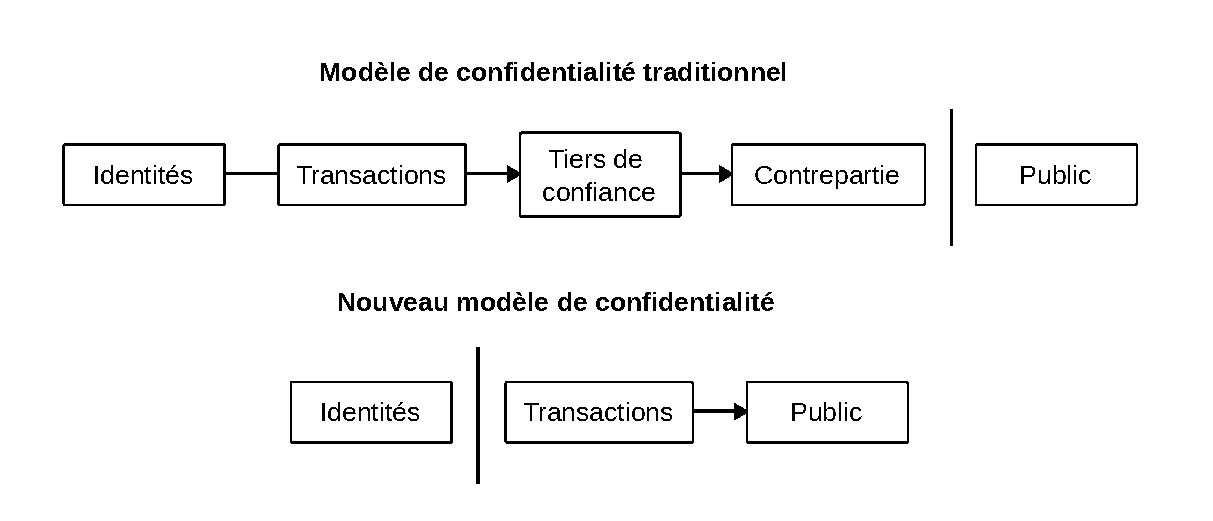
\includegraphics[scale=0.55]{img/white-paper-privacy-model-fr.eps}
  \caption{Modèle de confidentialité présenté dans le livre blanc de Bitcoin.}
\end{figure}

% Fuites d'information
Toutefois, des fuites d'information peuvent avoir lieu~: l'identité de l'utilisateur peut être dévoilée, que ce soit du fait de sa propre erreur ou de la divulgation (volontaire ou involontaire) de son interlocuteur dans l'échange. Par conséquent, nul ne peut prétendre être à l'abri de telles fuites\sendnote{Les premiers utilisateurs de Bitcoin ont ainsi été bien imprudents, à l'instar de Hal Finney qui a révélé des informations entre 2013 et 2014 permettant de déduire qu'il possédait plus de 10~000~bitcoins en 2011. -- Hal Finney, \emph{Bitcoin and me}, \wtime{19/03/2013 20:40:02 UTC}~: \url{https://bitcointalk.org/index.php?topic=155054.msg1643833\#msg1643833}~; Andy Greenberg, \eng{Nakamoto's Neighbor: My Hunt For Bitcoin's Creator Led To A Paralyzed Crypto Genius}, 25 mars 2014~: \url{https://www.forbes.com/sites/andygreenberg/2014/03/25/satoshi-nakamotos-neighbor-the-bitcoin-ghostwriter-who-wasnt/}.}. C'est pourquoi il existe des méthodes permettant de limiter leur effet et de retrouver la confidentialité en toute sérénité.

% Usage unique des adresses
La première mesure est l'usage unique des adresses. Elle consiste à générer une nouvelle clé privée et une nouvelle adresse lors de chaque paiement entrant et sortant. L'apport est de réduire l'impact de la révélation du lien avec l'identité sur la confidentialité générale~: tant que l'adresse n'est pas liée à d'autres par l'observation d'une action sur la chaîne (co-dépense par exemple), la fuite d'information se limite à cette seule adresse. Cette bonne pratique était citée dans le livre blanc\sendnote{«~Comme pare-feu supplémentaire, une nouvelle paire de clés devrait être utilisée pour chaque transaction afin de les empêcher d'être liées à un propriétaire commun. Certains liens sont toujours inévitables avec les transactions à entrées multiples, qui révèlent nécessairement que leurs entrées appartiennent au même propriétaire. Le risque est que si le propriétaire d'une clé est révélé, la liaison pourrait révéler d'autres transactions qui lui appartiennent.~» -- Satoshi Nakamoto, \eng{Bitcoin: A Peer-to-Peer Electronic Cash System}, 31 octobre 2008.} et est aujourd'hui implémentée dans tous les portefeuilles.

% Mélange de pièces
On peut également corriger les erreurs. Une des méthodes la plus connue pour procéder à ce type de correction est le mélange de pièces, qui permet de combiner ses UTXO avec d'autres utilisateurs afin de briser le lien déterministe qui existe.

% Tumblers
Le mélange de bitcoins était originellement pris en charge par des services de mixage centralisés, appelés \eng{mixers} ou \eng{tumblers}, qui recevaient les bitcoins des utilisateurs, les fusionnaient et leur renvoyaient des bitcoins communs au bout d'un certain temps, préférablement sous la forme de plusieurs transactions. Le premier mélangeur de ce type était BitLaundry, qui a été lancé en septembre 2010 par Peter Vessenes\sendnote{Peter Vessenes, \eng{Announcing: BitLaundry -- decorrelated payment service}, \wtime{01/09/2010 05:52:25 UTC}~: \url{https://bitcointalk.org/index.php?topic=963.msg11823\#msg11823}.}. Ces services permettaient d'obscurcir la provenance des bitcoins pour un observateur extérieur, mais pas pour le gérant du service, qui pouvait également voler les bitcoins au passage.  % Bitcoin Fog (2011), Silk Road

% CoinJoin
Une technique pour procéder à ce type de mélange sans devoir passer par un intermédiaire a par la suite été développée. C'était CoinJoin, dont la description formelle a été faite en août 2013 par Gregory Maxwell\sendnote{Gregory Maxwell, \eng{CoinJoin: Bitcoin privacy for the real world}, \wtime{22/08/2013 02:32:31 UTC}~: \url{https://bitcointalk.org/index.php?topic=279249.msg2983902\#msg2983902}.}. Il s'agit d'impliquer les pièces dans une transaction jointe collaborative qui brise la correspondance entre les entrées et une partie des sorties. La transaction classique que l'on se représente est celle de plusieurs utilisateurs qui signent chacun une entrée, dont la même nombre de sorties possèdent un montant égal, et dont le reste des sorties forment les sorties complémentaires. Dans ce cas, les sorties complémentaires sont toujours liées aux entrées, contrairement aux sorties principales qui sont indiscernables les unes des autres.

\textcolor{brown}{schéma transaction CoinJoin à 5 utilisateurs}

% Ensemble d'anonymat
Ces mélanges reposent sur la notion d'«~ensemble d'anonymat~» (\eng{anonymity set}) qui permet de mesurer la difficulté à faire le lien entre l'entrée et le sortie à un moment donné. On peut ainsi obtenir un score prospectif qui est le nombre de possibilités de pièces en sorties auxquelles peuvent correspondre un pièce en entrée. Dans notre exemple ci-dessus, le score prospectif de la sortie au moment de la transaction est de 5. Si la pièce avait subi un nouveau mélange (comme c'est fait dans Whirlpool), alors elle aurait eu un score prospectif de 9. On peut aussi, même si c'est plus rare, calculer un score rétrospectif qui correspond au nombre de potentielles pièces en entrée auxquelles peut être liée une sortie particulière, qui est également de 5 dans le cas de notre transaction simple, mais qui peut être largement supérieur en cas de remélanges fréquents. \sendnote{Loïc Morel, \emph{Comprendre et utiliser le CoinJoin sur Bitcoin}, 19 juillet 2022~: \url{https://www.pandul.fr/post/comprendre-et-utiliser-le-coinjoin-sur-bitcoin}.}

% Coordinateur
Pour gérer le tout, le système fait utilise généralement un protocole qui permet aux participants d'être mis en relation anonymement par le biais d'un coordinateur sans risque de fuite d'information ou de vol des fonds. Le plus connu est ZeroLink, développé par Adam Ficsor (\texttt{nopara73}) et \texttt{TDevD} en août 2017, qui est un protocole qui utilise le procédé de signature aveugle de David Chaum\sendnote{nopara73, TDevD, \eng{ZeroLink: The Bitcoin Fungibility Framework}, 14 août 2017~: \url{https://github.com/nopara73/ZeroLink/tree/32ad53927a343383534bea28fffb098af65fe62a}.}. C'est dans ce sens qu'on parle parfois de CoinJoin chaumien (\eng{Chaumian CoinJoin}). Une implémentation classique de cette idée a été réalisée par Whirlpool et par Wasabi 1.0. Des variantes (CoinShuffle, CoinShuffle++, CashShuffle, CashFusion) ont été implémentées sur des variantes de Bitcoin comme Decred ou Bitcoin Cash. Plus récemment le portefeuille Wasabi a intégré Wabisabi qui permet de réaliser des mélanges avec des valeurs arbitraires en sortie, ce qui complique l'estimation de la confidentialité apportée mais mais évite d'avoir à gérer les sorties complémentaires d'une manière séparée.

% PayJoin
Mais les transactions collaboratives ne se limitent pas au CoinJoin. Il existe par exemple une autre méthode, appelée PayJoin, qui permet au commerçant de réaliser un mélange avec le client au moment du paiement, en impliquant une pièce en entrée. Cela a pour effet de fausser l'analyse de chaîne en faisant croire à l'observateur extérieur qu'un seul utilisateur a réuni ses pièces en entrée.

Reprenons notre exemple d'Alice qui paie 7~mBTC à Bob en réunissant deux pièces de 6 et 1~mBTC afin d'atteindre un montant suffisant en entrée. Dans ce cas, les deux entrées sont supposément liées entre elles (heuristique de co-dépense) ainsi qu'à la sortie de 1~mBTC (heuristique de la sortie complémentaire). Dans ce cas, PayJoin consiste à faire en sorte que le commerçant inclue une ou plusieurs pièces en entrée et augmente d'autant le montant de la sortie qui lui est destinée.

\textcolor{brown}{schéma transaction à 3 entrées et 2 sorties}

Cette technique a été conceptualisée en 2018 sous la forme du protocole Bustapay proposé dans le BIP-79, qui n'a été mis en application. Elle a est néanmoins implémentée aujourd'hui par l'intermédiaire du protocole de paiement Pay-to-EndPoint (P2EP) implémenté dans plusieurs portefeuilles\sendnote{Adam Ficsor, \eng{Pay To EndPoint}, 31 juillet 2018~: \url{https://nopara73.medium.com/pay-to-endpoint-56eb05d3cac6}.} et des transactions Stowaway du Samourai Wallet\sendnote{Samourai Wallet, \eng{Stowaway}~: https://samouraiwallet.com/stowaway}.

% CoinSwap
Enfin une dernière méthode est Coinswap, qui est un procédé développé par Chris Belcher, qui permet à deux utilisateurs ou plus d'échanger leurs pièces sans qu'ils aient besoin de se faire confiance et sans que cette opération laisse une trace particulière sur la chaîne\sendnote{Chris Belcher, \eng{Design for a CoinSwap Implementation for Massively Improving Bitcoin Privacy and Fungibility}, 25 mai 2020~: \url{https://gist.github.com/chris-belcher/9144bd57a91c194e332fb5ca371d0964}.}.

\section*{La machine virtuelle}
\addcontentsline{toc}{section}{La machine virtuelle}

% Monnaie programmable
Les scripts présents au sein des transactions font de Bitcoin un système de monnaie programmable. Ces scripts permettent en effet la mise en place d'une variété de conditions de dépense, aussi appelées clauses, qui vont au-delà de l'exigence d'une signature simple, comme la connaissance d'un secret, l'attente d'une période de temps ou la production de signatures multiples.

% Machine abstraite répliquée, machine virtuelle, machine à états
La mise en œuvre de Bitcoin crée une machine abstraite dont le fonctionnement est répliqué sur tous les nœuds du réseau grâce à l'algorithme de consensus. Elle est simulée par l'intermédiaire de l'implémentation logicielle, de sorte qu'on parle de machine virtuelle. Plus précisément, il s'agit d'un machine à états, dont l'état courant est l'ensemble des pièces existantes, c'est-à-dire l'ensemble des sorties transactionnelles non dépensées (UTXO), et dont les transitions sont les transactions, qui détruisent des pièces pour en créer de nouvelles. Ces transactions sont assemblées dans des blocs qui sont validés à intervalles réguliers par les mineurs. La diffusion d'un bloc sur le réseau permet d'actualiser l'état de la machine virtuelle, qui est la plupart du temps partagé par tous les nœuds.

% réplication de machine à états (\eng{state machine replication})
% FAUX : automate fini (appelé \eng{finite-state machine} en anglais) qui peut être dans une quantité finie d'états, mais qui n'est, à un moment donné, que dans un seul état\sendnote{Contrairement à ce qui est parfois affirmé, la machine virtuelle n'est pas un automate à deux piles (\eng{dual-stack pushdown automaton}), même si le langage de programmation interne en émule un. -- Craig S. Wright, \eng{Beyond Godel}, 2018~: \url{https://coingeek.com/wp-content/uploads/2018/03/SSRN-id3147440.pdf}.}. Même s'il est très grand, l'ensemble des états possibles est nécessairement fini en raison du codage des entiers sur 8 octets et de la limite de taille des scripts\sendnote{La limite de taille des scripts est actuellement de 10~ko sur BTC~: \url{https://github.com/bitcoin/bitcoin/blob/v0.17.0/src/script/script.h\#L31-L32}.}.

% Exécution des scripts
Au sein d'une transaction, le déverrouillage des pièces se fait par l'exécution de scripts. Les scripts sont des prédicats au sens mathématique, c'est-à-dire des expressions incomplètes qui deviennent des propositions pouvant être évaluées si elles sont complétées par un ou plusieurs éléments. De ce fait, la dépense consiste à réunir le script de verrouillage de la sortie précédente et le script de déverrouillage, et à les exécuter l'un après l'autre~: le script de déverrouillage d'abord, le script de verrouillage ensuite. L'utilisation de la pièce comme entrée de transaction n'est approuvée que si l'exécution réussit.

% Langage de programmation (règles de transition)
Les scripts sont écrits dans le langage de programmation interne de Bitcoin, conçu par Satoshi Nakamoto dès 2008 et baptisé de façon peu originale «~Script~». Ce langage de programmation fonctionne de manière similaire à Forth, un langage utilisé dans les années 1970 et 1980. Il se base en particulier sur deux piles de données, qui sont des structures de données fondées sur le principe du «~dernier arrivé, premier sorti~» (de l'anglais \eng{last in, first out}, abrégé en LIFO). Le langage agit essentiellement sur la pile primaire, de sorte que cette dernière est la plus importante~; la pile secondaire permet seulement de mettre des données de côté pendant l'exécution d'un script.

% Description par Satoshi
Satoshi Nakamoto a inclus ce système de scripts dans Bitcoin pour lui permettre de gérer une grande variété de cas d'utilisation. En juin 2010, en réponse à Gavin Andresen, il écrivait ainsi sur le forum~:

\begin{quote}
«~La nature de Bitcoin est telle que, dès la version 0.1 lancée, son fonctionnement de base était gravé dans le marbre pour le reste de son existence. C'est pour cette raison que je voulais concevoir Bitcoin pour qu'il supporte tous les types de transaction auxquels je pouvais penser. Le problème était que chaque élément requérait un code de prise en charge et des champs de données spéciaux, qu'il soit utilisé ou non, et ne pouvait couvrir qu'un cas particulier à la fois. Ç'aurait été une explosion de cas particuliers. La solution était script, qui généralisait le problème de façon à ce que les parties contractantes puissent décrire leurs transactions comme des prédicats que les nœuds du réseau évaluaient. Les nœuds ont seulement besoin de comprendre la transaction dans la mesure où ils évaluent si les conditions de l'émetteur sont remplies ou non.\sendnote{Satoshi Nakamoto, \eng{Re: Transactions and Scripts: DUP HASH160 ... EQUALVERIFY CHECKSIG}, \wtime{17/06/2010 18:46:08}~: \url{https://bitcointalk.org/index.php?topic=195.msg1611\#msg1611}.}~»
\end{quote} % "The nature of Bitcoin is such that once version 0.1 was released, the core design was set in stone for the rest of its lifetime.  Because of that, I wanted to design it to support every possible transaction type I could think of.  The problem was, each thing required special support code and data fields whether it was used or not, and only covered one special case at a time.  It would have been an explosion of special cases.  The solution was script, which generalizes the problem so transacting parties can describe their transaction as a predicate that the node network evaluates.  The nodes only need to understand the transaction to the extent of evaluating whether the sender's conditions are met."

% Opérateurs
Le langage est constitué de plus d'une centaine d'opérateurs, aussi appelés codes opération (ou \eng{opcodes} en anglais), qui agissent sur la pile primaire d'une manière ou d'une autre\sendnote{La liste des opérateurs et de leurs actions est disponible sur la page de Bitcoin Wiki consacrée à Script~: \url{https://en.bitcoin.it/wiki/Script}.}. Les opérateurs sont des nombres codés sur 1 octet (allant de 0 à 255), mais sont usuellement désignés par un nom décrivant leur fonction, dans le but de rendre la lecture plus compréhensible par l'être humain. Ils sont notés en majuscules et sont souvent précédés du préfixe \texttt{OP\_} même s'il peut être omis en l'absence d'ambiguïté. Par exemple, l'opérateur permettant de vérifier une signature (\texttt{0xac}) est noté \texttt{OP\_CHECKSIG} ou \texttt{CHECKSIG}.

% Empilement
Les opérateurs allant de 1 à 75, parfois notés \texttt{OP\_PUSHBYTES\_X}, ont pour action d'empiler des données ayant une taille allant de 1 à 75 octets. L'utilisation d'opérateurs supplémentaires spécifiques (notés \texttt{OP\_PUSHDATA\_Y}) permet cependant de placer une information plus grande sur la pile. Bien qu'on puisse utiliser cette notation, il est généralement plus simple de placer un élément entre chevrons pour indiquer qu'il est placé au sommet de la pile. Par exemple, le fait d'écrire \texttt{<signature>} au sein d'un script signifie que la signature est empilée.

% Valeur retournée
La valeur retournée à la fin de l'exécution des scripts est un booléen, de sorte que le script peut être valide, auquel cas la dépense de la pièce est approuvée, ou bien invalide, auquel cas la transaction est rejetée dans son ensemble. Le script est valide si et seulement si la valeur \texttt{TRUE} («~vrai~» en anglais) est présente en haut de la pile à la fin de l'exécution. Il est invalide si ce n'est pas le cas ou si son exécution s'est arrêtée avant la fin.

% Pas de boucles
Le langage Script est cependant limité. Rien dans sa conception ne permet pas de faire de boucles, ni d'accéder à des données extérieures à celles de la transaction, contrairement au langage d'Ethereum qui est quasi Turing-complet. Cette particularité fait qu'il est moins flexible, mais qu'il a l'avantage d'être plus simple à appréhender et donc plus sûr.

% Exemple : vérification d'une addition (38 = 17 + x)
L'exemple typique de script, présenté par Andreas Antonopoulos\sendnote{Andreas Antonopoulos, \eng{Mastering Bitcoin (second edition)}, ch.6, 2017.}, est celui qui consiste à résoudre une équation simple impliquant une addition. Si on considère l'équation $17 + x = 38$, alors le script de verrouillage qui correspond est~:

\begin{Verbatim}[fontsize=\small]
<17> ADD <38> EQUAL
\end{Verbatim}

Toute personne disposant de la réponse peut dépenser la pièce, ce qui on en convient n'est pas très sécurisé. La dépense requiert ici de fournir le script de déverrouillage composé uniquement de la solution de l'équation, à savoir 21~:

\begin{Verbatim}[fontsize=\small]
<21>
\end{Verbatim}

L'exécution successive de ces deux scripts a lieu comme suit~: 1)~la valeur 17 est placée sur la pile~; 2)~la valeur 21 est placée au-dessus~; 3)~l'opérateur \texttt{OP\_ADD} additionne les deux valeurs en haut de la pile et les remplace par leur somme, ici 38~; 4)~la valeur 38 est placée au sommet de la pile~; 5)~l'opérateur \texttt{OP\_EQUAL} compare les deux valeurs en haut de la pile et les remplace par le booléen d'égalité, ici \texttt{TRUE}. L'exécution du script est donc un succès.

\textcolor{brown}{schéma exécution du script et données sur la pile}

Si la valeur avait été différente, 22 par exemple, alors la dernière opération aurait retourné le booléen \texttt{FALSE} et la transaction de dépense aurait été invalidée.

% --- Exemples de scripts complets ---

Beaucoup de conditions de dépense différentes peuvent être implémentées par ce système. Certaines de ces conditions sont simples comme la connaissance d'un secret spécifique ou la production d'une signature valide correspondant à une clé publique particulière.

La connaissance d'un secret (dont l'empreinte est spécifiée dans l'UTXO) est vérifiée par les scripts suivants qui placent le secret au sommet de la pile, le hachent par SHA-256 et comparent le résultat à l'empreinte~:

\begin{Verbatim}[fontsize=\small]
<secret> || SHA256 <empreinte> EQUAL
\end{Verbatim}

De même, la vérification de la validité d'une signature est réalisée par les scripts suivants qui empilent d'abord la signature, puis la clé publique avant de contrôler leur correspondance~:

\begin{Verbatim}[fontsize=\small]
<signature> || <clé publique> CHECKSIG
\end{Verbatim}

% Verrous temporels
Mais il existe des conditions plus avancées comme les verrous temporels. Ceux-ci permettent de bloquer les fonds de la pièce pour un temps précis, que ce soit jusqu'à une date donnée, auquel cas on parle de temps de verrouillage absolu, ou bien pendant une période donnée, auquel cas on parle de temps de verrouillage relatif. Le premier est le fait de l'opérateur \texttt{OP\_CHECKLOCKTIMEVERIFY} dont les spécificités techniques sont décrites dans le BIP-65. Le second est appliqué par le code opération \texttt{OP\_CHECKSEQUENCEVERIFY} décrit dans le BIP-112.

% DESCRIPTION TECHNIQUE
%
% Les scripts suivants vérifient un temps de verrouillage absolu, c'est-à-dire lié à une date particulière~:
%
% \begin{verbatim}
% TRUE || <date de verrouillage> CHECKLOCKTIMEVERIFY DROP
% \end{verbatim}
%
% Le booléen \verb?TRUE? est mise en haut de la pile. Puis, est empilée la date jusqu'à laquelle le verrouillage persiste, qui est donnée en horodatage MTP ou en hauteur de blocs. Ensuite, cette date est comparée à la date indiquée dans le champ \verb?nLocktime? de la transaction, qui est elle-même comparée à l'horodatage du réseau. Enfin, la date est expulsée de la pile, ce qui fait qu'il ne reste que le booléen \verb?TRUE? sur la pile.
%
% Les scripts suivants vérifient un verrou temporel relatif, qui est lié à la période de temps écoulée depuis la date de confirmation de la pièce~:
%
% \begin{verbatim}
% TRUE || <période de verrouillage> CHECKSEQUENCEVERIFY DROP
% \end{verbatim}
%
% Le booléen \verb?TRUE? est mise en haut de la pile. Puis, c'est au tour de la période de verrouillage, qui est donnée en secondes\sendnote{Ou plus précisément en unités de 512 secondes.} ou en nombre de blocs. Ensuite, cette période est comparée à la période de temps indiquée dans le champ \verb?nSequence? de l'entrée dépensant la pièce, qui est elle-même comparée à la période de temps écoulée depuis la date de confirmation de la pièce. Enfin, la période est expulsée de la pile, ne laissant que le booléen \verb?TRUE? au sommet de la pile.
%
% Ce fonctionnement un peu plus compliqué des verrous temporels s'explique par le fait qu'ils ont été intégrés sous la forme de soft fork.


\section*{Les schémas classiques}
\addcontentsline{toc}{section}{Les schémas classiques}

% --- Schémas et règles de mempool ---

Le langage Script permet de faire des choses diverses et variées. Pendant les premiers temps de Bitcoin, le système était relativement libre et autorisait les gens à écrire ce qu'ils voulaient dans les scripts sans discrimination. Toutefois, cette situation était considérablement risquée. La raison principale était que le fonctionnement des codes opération n'était pas encore vérifié et testé, comme l'a montré la découverte en juillet 2010 d'une vulnérabilité rendue possible par certains opérateurs binaires\sendnote{NIST, \eng{CVE-2010-5137}, 8 juin 2012~: \url{https://nvd.nist.gov/vuln/detail/CVE-2010-5137}.}. C'est pourquoi il a été décidé à la fin de l'année 2010, sous l'impulsion de Gavin Andresen, de restreindre la facilité de programmation du système\sendnote{Gavin Andresen, \eng{svn r197: IsStandard check for transactions}, \wtime{07/12/2010 13:58:33 UTC}~: \url{https://bitcointalk.org/index.php?topic=2129.msg27744\#msg27744}.}.

% Schémas standards
Cette restriction a été appliquée en imposant des schémas standards de scripts, qui faisaient que les nœuds configurés par défaut ne relayaient plus les transactions contenant des scripts qui ne respectaient pas ce standard. Il ne s'agissait pas ainsi d'une restriction des règles globales de consensus, mais des règles locales de mempool qui s'applique à la transmission des transactions. Des schémas standards rendant les choses plus simples et plus sûres ont ainsi été développés au cours des années. Les schémas standards de sortie transactionnelle étaient \textcolor{darkgray}{en 2023} au nombre de huit~: P2PK, P2PKH, P2MS, P2SH, NULLDATA, P2WPKH, P2WSH et P2TR\sendnote{\url{https://github.com/bitcoin/bitcoin/blob/22.x/src/script/standard.h\#L59-L71}.}.

% --- Pay to Public Key ---

\textbf{P2PK~: Pay to Public Key} Le premier schéma s'appelle Pay to Public Key (P2PK), qu'on peut traduire littéralement en français par «~payer à la clé publique~». Il s'agit de créer une pièce liée à la clé publique d'un destinataire, que lui seul peut dépenser en signant avec sa clé privée. Le script de verrouillage permettant ce type d'envoi est~:

\begin{Verbatim}[fontsize=\small]
<clé publique> CHECKSIG
\end{Verbatim}

La présence de la clé publique explique qu'on parle parfois de «~scriptPubKey~» pour désigner le script de verrouillage en général, indépendemment de ce qu'il contient.

Au moment de la dépense, le destinataire doit utiliser un script de déverrouillage contenant simplement sa signature~:

\begin{Verbatim}[fontsize=\small]
<signature>
\end{Verbatim}

La présence de la signature dans ce script explique qu'on parle parfois de «~scriptSig~» pour désigner le script de déverrouillage en général, indépendemment de ce qu'il contient.

L'exécution successive de ces deux scripts permet, comme on l'a vu, de vérifier que la signature fournie par l'utilisateur correspond à sa clé publique, auquel cas elle est valide.

Le schéma P2PK était utilisé dans les débuts de Bitcoin pour recevoir les paiements par IP (P2IP) et pour récupérer la récompense de minage. Il est aujourd'hui tombé en désuétude au profit d'un schéma rival~: P2PKH.

% --- Pay to Public Key Hash --

\textbf{P2PKH~: Pay to Public Key Hash.} Le schéma Pay to Public Key Hash (P2PKH), qui est traduit littéralement par «~payer à l'empreinte de la clé publique~», est le deuxième type de format de réception apparu dans Bitcoin dès le début du fait de la conception de Satoshi Nakamoto. Ce schéma permet non pas de réaliser un paiement vers une clé publique, mais vers l'empreinte d'une clé publique, tout en faisant en sorte que l'interpréteur vérifie quand même la validité de la signature vis-à-vis de la clé publique lors de la dépense des fonds. L'empreinte de la clé publique est alors considérée comme la donnée essentielle de l'adresse, qui dans ce cas commence toujours par un 1, comme par exemple \longstring{1FjBKPQ7MTiPSDkJ2ZwPgAXUKQ8yoGbVJX}.

Le script de verrouillage ici est~:

\begin{Verbatim}[fontsize=\small]
DUP HASH160 <empreinte de la clé publique> EQUALVERIFY CHECKSIG
\end{Verbatim}

Et le script de déverrouillage est~:

\begin{Verbatim}[fontsize=\small]
<signature> <clé publique>
\end{Verbatim}

L'exécution des deux scripts permet de~: 1) vérifier que le passage de la clé publique par la fonction de hachage HASH-160 est égale à l'empreinte qui est spécifiée dans le script ; 2) vérifier la signature correspond à la clé publique.

L'avantage de ce schéma est qu'il permet d'avoir des adresses plus courtes (l'information à encoder n'est que de 20~octets au lieu de 65~octets pour une clé publique), raison pour laquelle Satoshi Nakamoto l'a implémenté. De plus, en ne révélant la clé publique qu'au moment de la dépense, ce schéma accroît aussi la sécurité contre la menace (très hypothétique) de l'ordinateur quantique.

% --- Pay To MultiSig ---

\textbf{P2MS~: Pay To MultiSig.} Le schéma Pay To MultiSig (P2SH), qui signifie littéralement «~payer à la multisignature~», est un schéma exigeant la signature de M personnes parmi N participants prédéterminés («~M-parmi-N~», ou «~M-of-N~» en anglais). Il a été rendu standard sous une forme limitée à 3 participants en mars 2012 avec la sortie de la version 0.6.0 du logiciel\sendnote{Gavin Andresen, \eng{Version 0.6.0 released}, 30 mars 2012~: \url{https://bitcointalk.org/index.php?topic=74737.msg827484\#msg827484}.}. Le script de verrouillage est le suivant~:

\begin{Verbatim}[fontsize=\small]
M <clé publique 1> ... <clé publique N> N CHECKMULTISIG
\end{Verbatim}

Le script de déverrouillage correspondant est~:

\begin{Verbatim}[fontsize=\small]
<leurre (0)> <signature 1> ... <signature M>
\end{Verbatim}

La présence du leurre (généralement 0) est dû à un défaut dans l'implémentation de l'exécution de l'opérateur \texttt{OP\_CHECKMULTISIG} par Satoshi, qui requiert un élément de trop. Les développeurs n'ont pas jugé rentable de corriger ce défaut, car cette correction constituait un hard fork.

C'est ce schéma, particulièrement exigeant au niveau de la mise en place, qui a motivé la création du schéma P2SH.

\textbf{P2SH : Pay to Script Hash} Le schéma Pay to Script Hash (P2SH), pouvant être traduit littéralement par «~payer à l'empreinte du script~», reprend l'idée derrière P2PKH, à la seule différence que la donnée hachée n'est pas une clé publique, mais le script lui-même~! Le script en question est alors appelé script de récupération (\eng{redeem script}) pour le différencier du script de déverrouillage. Son empreinte est la donnée constituante de l'adresse, cette dernière commençant toujours par un 3 à l'instar de \longstring{3K8Ps6Ayw5ZaKDaLZjfGo3mTgDsc1VXZ8d}.

% \sendnote{Ludovic Lars, \emph{Pay to Script Hash (P2SH) pleinement expliqué}, 14 juillet 2020~: \url{https://viresinnumeris.fr/pay-to-script-hash-p2sh-pleinement-explique/}.}

Ce schéma donne à l'utilisateur la possibilité d'y inclure n'importe quel script, sans discrimination sur son format, à condition qu'il respecte bien sûr certaines limites. Il permet aussi de recevoir des fonds depuis la quasi-totalité des portefeuilles existants, le fardeau de la construction et du déverrouillage du script revenant uniquement au destinataire, et pas aussi à l'expéditeur comme c'est le cas dans le scripting brut.

Le script de verrouillage pour le schéma P2SH est~:

\begin{Verbatim}[fontsize=\small]
HASH160 <empreinte du script de récupération> EQUAL
\end{Verbatim}

Et le script de déverrouillage est un script de la forme~:

\begin{Verbatim}[fontsize=\small]
[éléments de déverrouillage] <script de récupération>
\end{Verbatim}

L'exécution de P2SH est plus complexe que les précédents schémas, ce qui peut s'expliquer par le contexte dans lequel il a été développé. L'idée d'implémenter un schéma de script qui utilise l'empreinte d'un autre script comme l'empreinte de clé publique dans le schéma P2PKH est née 2011 en faisant l'objet de plusieurs propositions\sendnote{Mike Caldwell (casascius), \eng{Proposal to modify OP\_CHECKSIG}, \wtime{22/09/2011 02:21:17 UTC}~: \url{https://bitcointalk.org/index.php?topic=45211.msg538756\#msg538756}~; jimrandomh, \eng{Proposed extensions to the transaction protocol: Receiver scripts, OP\_TIME, more}, \wtime{01/10/2011 16:56:47 UTC}~: \url{https://bitcointalk.org/index.php?topic=46429.msg553217\#msg553217}~; Gavin Andresen, \eng{Re: Proposal to modify OP\_CHECKSIG}, \wtime{02/10/2011 00:26:42 UTC}~: \url{https://bitcointalk.org/index.php?topic=45211.msg553668\#msg553668}.}. Elle a été rendue plus concrète avec une proposition de l'opérateur \texttt{OP\_EVAL} par Nicolas van Saberhagen le 2 octobre, code opération qui permettait l'exécution récursive d'un script à l'intérieur d'un autre script\sendnote{Nicolas van Saberhagen, \eng{OP\_EVAL proposal}, \wtime{02/10/2011 00:49:19 UTC}~: \url{https://bitcointalk.org/index.php?topic=46538.msg553689\#msg553689}.}. Gavin Andresen a expliqué comment en faire un soft fork par le remplacement de l'instruction sans effet \texttt{OP\_NOP1}\sendnote{Gavin Andresen, \eng{Re: OP\_EVAL proposal}, \wtime{02/10/2011 20:42:32 UTC}~: \url{https://bitcointalk.org/index.php?topic=46538.msg554620\#msg554620}.}.

L'opérateur \texttt{OP\_EVAL} devait permettre de former un nouveau schéma standard. Le script de verrouillage aurait été~:

\begin{Verbatim}[fontsize=\small]
DUP HASH160 <empreinte du script de récupération> EQUALVERIFY EVAL
\end{Verbatim}

tandis que le script de déverrouillage aurait été le même. L'exécution successive de ces deux scripts aurait permis dans un premier temps de vérifier la conformité du hachage du script de récupération à l'empreinte~; puis dans un second temps d'exécuter le script de récupération et de lui combiner les éléments de déverrouillage.

Néanmoins cette solution n'a pas été acceptée, celle-ci ayant été jugée trop dangereuse à cause de son pouvoir de récursion. Il lui a été préféré le modèle plus restrictif de P2SH.

L'exécution de P2SH fonctionne exactement comme le schéma lié à \texttt{OP\_EVAL}, à l'exception qu'une partie du script n'est pas explicitement indiquée. D'une part, la vérification de la correspondance entre l'empreinte indiquée et le script de récupération est bien réalisée par le script de verrouillage. D'autre part, l'évaluation du script de récupération est effectuée implicitement grâce à une exception ajoutée au code source qui fait que les nœuds du réseau qui reconnaissent le schéma l'interprètent différemment. Dans Bitcoin Core, on peut observer cette condition au sein de la fonction \texttt{VerifyScript} de l'interpréteur\sendnote{\url{https://github.com/bitcoin/bitcoin/blob/22.x/src/script/interpreter.cpp\#L2018-L2062}}.

% Laideur
La proposition a été codifiée dans le BIP-16. Si cette solution est pratique, elle crée de la complexité et n'est pas très élégante. Comme le disait Gavin Andresen dans l'explication du BIP-16~:

\begin{quote}
«~Reconnaître une forme "spéciale" de scriptPubKey et réaliser une validation supplémentaire quand elle est détectée, c'est laid. Cependant, l'avis général est que les alternatives sont soit encore plus laides, soit plus complexes à implémenter, et/ou étendent le pouvoir du langage d'expression de manière dangereuse.\sendnote{Gavin Andresen, \eng{BIP-16: Pay to Script Hash}, 3 janvier 2012~: \url{https://github.com/bitcoin/bips/blob/master/bip-0016.mediawiki\#rationale}.}~»
\end{quote}

Le schéma P2SH a été activé le 1\ier{} avril 2012 sous la forme d'un soft fork, en dépit de l'opposition notable de luke-jr qui proposait un opérateur alternatif, \texttt{OP\_CHECKHASHVERIFY}, décrit dans le BIP-17\sendnote{Amir Taaki, \eng{The Truth behind BIP 16 and 17}, 29 janvier 2012~: \url{http://bitcoinmedia.com/the-truth-behind-bip-16-and-17/}~; archive~: \url{https://web.archive.org/web/20120202032835/http://bitcoinmedia.com/the-truth-behind-bip-16-and-17/}.}.

\section*{Les types de signature}
\addcontentsline{toc}{section}{Les types de signature}

% --- Types de signature ---

La programmabilité de Bitcoin n'est pas seulement issue de son langage de programmation mais aussi du système de signature qui permet de de sélectionner quelle partie de la transaction est signée. Ce facteur de programmabilité est mis en œuvre par l'existence d'un indicateur, appelé type de hachage de la signature ou \eng{signature hash type}, qui est ajouté à la transaction non signée, puis à la signature elle-même. Celui-ci indique quelle partie de la transaction doit être hachée avant d'être soumise à l'algorithme de signature, d'où son nom.

Le type de signature est construit à partir de plusieurs signaux de signature qui peuvent être combinés. Les quatre signaux de signature qui existent sont~:

\begin{itemize}
\item[$\bullet$] \texttt{SIGHASH\_ALL} (\texttt{0x01}) qui indique que toutes les sorties sont signées~;
\item[$\bullet$] \texttt{SIGHASH\_SINGLE} (\texttt{0x03}) qui permet de ne signer qu'une seule sortie~;
\item[$\bullet$] \texttt{SIGHASH\_NONE} (\texttt{0x02}) qui indique qu'aucune sortie n'est signée~;
\item[$\bullet$] \texttt{SIGHASH\_ANYONECANPAY} (\texttt{0x80}) qui permet de ne signer qu'une seule entrée.
\end{itemize}

Les trois signaux concernant les sorties peuvent être associés à \texttt{SIGHASH\_ANYONECANPAY}, ce qui permet de former finalement six types de signatures différents. Le type de signature le plus fréquent est évidemment \texttt{SIGHASH\_ALL} même si certains autres types peuvent parfois trouver une utilité. C'est notamment le cas de \texttt{SIGHASH\_ALL | SIGHASH\_ANYONECANPAY} qui permet de construire des transactions de type \eng{anyone-can-pay}, dont les sorties sont déterminées, mais où chacun peut signer sa propre entrée sans connaître les autres.

\textcolor{brown}{schéma types de signature}

% Notez que tout ceci était présent dès la création de Bitcoin et que Satoshi Nakamoto avait intégré ce type de signature dans le code d'origine.

% SIGHASH_NOINPUT
Ces signaux ont été implémentés dès le début par Satoshi Nakamoto au sein du prototype. Il en manquait logiquement un, que Satoshi Nakamoto a probablement jugé inutile~: celui qui ne signait aucune entrée. Toutefois, avec le développement des canaux de paiements pour le réseau Lightning, les développeurs se sont rendus compte qu'il pouvait avoir une utilité. C'est dans cet esprit que le signal de signature \texttt{SIGHASH\_NOINPUT} a été proposé en février 2016 par Joseph Poon\sendnote{Joseph Poon, \eng{[bitcoin-dev] SIGHASH\_NOINPUT in Segregated Witness}, \wtime{26/02/2016 01:07:46 UTC}~: \url{https://lists.linuxfoundation.org/pipermail/bitcoin-dev/2016-February/012460.html}.}.

% BIP-118, SIGHASH_ANYPREVOUT
Ce type de signal pourrait être implémenté de manière partielle dans BTC au travers du BIP-118, qui prévoit l'implémentation de deux nouveaux signaux -- \texttt{SIGHASH\_ANYPREVOUT} et \texttt{SIGHASH\_ANYPREVOUTANYSCRIPT} -- au sein des scripts de Taproot\sendnote{Christian Decker, Anthony Towns, \eng{BIP-118: SIGHASH\_ANYPREVOUT for Taproot Scripts}, 28 février 2017~: \url{https://github.com/bitcoin/bips/blob/master/bip-0118.mediawiki}.}. Il permettrait d'améliorer le fonctionnement du réseau Lightning par la mise en œuvre du protocole Eltoo qui repose sur la construction de transactions flottantes.

\section*{SegWit~: le témoin séparé}
\addcontentsline{toc}{section}{SegWit~: le témoin séparé}

% Présentation de SegWit
SegWit, abréviation de \eng{Segregated Witness}, qu'on peu traduire littéralement par «~témoin séparé~», est une mise à niveau du protocole ayant lieu sur LTC et sur BTC en 2017. Elle a consisté à faire en sorte que les données de déverrouillage des entrées transactionnelles, telles que les signatures, se retrouvent dans une structure de données séparée (\eng{segregated}) appelée le témoin (\eng{witness}) afin de supprimer la malléabilité des transactions. SegWit constituait ainsi une restructuration profonde des transactions.

% Autres apports
Outre la correction de la malléabilité, SegWit a apporté une augmentation de capacité transactionnelle et un versionnage des scripts pour faciliter les mises à niveau ultérieures. Elle a également amélioré l'algorithme de signature pour éviter les hachages redondants durant la vérification et pour rendre plus sûre la signature hors-ligne\sendnote{Voir BIP-143~: \url{https://github.com/bitcoin/bips/blob/master/bip-0143.mediawiki}.}.

% --- Malléabilité ---

\textbf{Malléabilité.} SegWit tire son origine du problème de la malléabilité des transactions, un problème qui est identifié depuis janvier 2012\sendnote{Gavin Andresen, \eng{[Bitcoin-development] Extending IsStandard() to transaction scriptSigs}, \wtime{19/1/2012 16:29:29}, \url{https://lists.linuxfoundation.org/pipermail/bitcoin-dev/2012-January/001066.html}.}. Dans Bitcoin, les transactions sont malléables dans le sens où elles peuvent être modifiées légèrement après leur diffusion sans devenir invalides aux yeux du réseau. Cette propriété vient du fait qu'une signature ne peut pas se prendre en compte elle-même et que par conséquent le script de déverrouillage n'est pas signé avec le reste de la transaction. La malléabilité peut ainsi prendre deux formes~: la malléabilité intrinsèque à l'algorithme ECDSA, qui se base sur un nombre aléatoire pour produire une signature (malléabilité par le signataire)~; la malléabilité provenant de la forme des signatures et des scripts de déverrouillage des entrées (malléabilité par un tiers).

% Problèmes
La malléabilité n'est pas rédhibitoire pour la sécurité des fonds, mais elle permet de modifier l'identifiant de la transaction après sa publication, ce qui peut se révéler problématique dans certaines situations. Ainsi, entre le 9 et le 11 février 2014, Mt. Gox et d'autres plateformes d'échange ont subi des attaques exploitant cette malléabilité des transactions\sendnote{Ken Shirriff, \eng{The Bitcoin malleability attack graphed hour by hour}, 15 février 2014~: \url{https://www.righto.com/2014/02/the-bitcoin-malleability-attack-hour-by.html}}. Les transactions de retrait ont été modifiées par les attaquants, faisant croire aux plateformes mal configurées que ces transactions n'avaient pas été confirmées, ce qui leur a permis de recréditer leur compte tout en conservant les bitcoins. Ces attaques ont mené à une perte totale de 64~564~bitcoins\sendnote{Christian Decker, Roger Wattenhofer, \eng{Bitcoin Transaction Malleability and MtGox}, 26 mars 2014~: \url{https://arxiv.org/pdf/1403.6676.pdf\#page=8}.}.

% Tentatives de correction
Des propositions ont tenté de corriger la malléabilité par un tiers en contraignant au maximum la forme des transactions. C'est dans cet esprit que le BIP-62 a été créé en mars 2014, dont l'une des exigences (l'encodage standard des signatures décrit dans le BIP-66) a été incluse dans les règles de consensus le 4 juillet 2015. Toutefois, ces changements ne s'appliquaient pas à la malléabilité par le signataire, ce qui créait la demande pour une correction généralisée.

% Lightning Network
Cette malléabilité signifiait que tout acteur participant à un schéma de multisignature pouvait modifier la transaction et donc son identifiant à tout moment. Cela altérait significativement la possibilité d'implémentation du réseau Lightning, dont les canaux de paiements, comme on le verra plus bas, se basent sur des transactions non publiées auxquelles il faut faire référence et font intervenir des signatures multiples.

% Solution : séparer les signatures du reste de la transaction
La solution était de mettre de côté les scripts de déverrouillage dans le processus de hachage de la transaction, pour qu'un changement de ces scripts n'influence pas l'identifiant. Cette idée a été proposée initialement par Gregory Maxwell en août 2013 sur IRC\sendnote{«~Je suggère de ne jamais hacher cette valeur dans le protocole. En gros, je dis que les scriptsigs pour une [transaction] seraient un arbre de hachage séparé. Il est toujours engagé dans la chaîne de blocs mais ce serait une branche séparée.~» -- Gregory Maxwell, IRC, \wtime{29/08/2013 20:21 UTC}~: \url{https://download.wpsoftware.net/bitcoin/wizards/2013/08/13-08-29.log}.}, avant d'être mise en œuvre au sein de la version alpha du modèle de sidechain appelé Elements, annoncée le 8 juin 2015 par Blockstream\sendnote{\url{https://blog.blockstream.com/en-714/}}. Le même jour, Gregory Maxwell présentait cette version d'Elements incluant \eng{Segregated Witness} dans un séminaire de développements de San Francisco~: il décrivait alors le témoin comme «~une valeur spécifique qui constitue une preuve concrète d'affirmation existentielle\sendnote{\url{https://www.youtube.com/watch?v=Twynh6xIKUc}~; \url{https://mirror.explodie.org/blockstream.gmaxwell.elements.talk.060815.pdf}.}~».

% 20:21 < gmaxwell> e.g. OP_NOP <push> checksig is still valid.. so you'd have to have a rule saying you couldn't do that.  But I'm suggesting never hashing that value anywhere in the protocol.
% 20:21 < gmaxwell> basically I'm saying the scriptsigs for a txn would be a seperate hashtree. You'd still commit it in the blockchain but it would be a seperate fork.

% SegWit en tant que proposition d'amélioration de Bitcoin
Cette solution a été adaptée pour Bitcoin au cours de l'automne 2015, pour être appliquée comme un soft fork. La mise à niveau SegWit a été officiellement introduite à la communauté par le développeur Pieter Wuille le 7 décembre 2015, lors de la conférence Scaling Bitcoin \textsc{II} à Hong Kong. En substance, elle consistait à déplacer les scripts de déverrouillage dans le témoin de la transaction. Deux identifiants étaient alors calculés~: l'identifiant classique (\texttt{txid}), qui ne prend pas en compte ce témoin, et l'identifiant complet (noté \texttt{wtxid} pour \eng{witness transaction identifier}), qui recouvre l'intégralité de la transaction. Les identifiants complets étaient regroupés dans un second arbre de Merkle, dont la racine était placée dans la transaction de récompense du bloc, ce qui faisait que toutes les données étaient engagées dans le calcul de la preuve de travail. De l'autre côté, les transactions et les blocs restaient valides pour les nœuds n'ayant pas été mis à niveau.

% Correction de la malléabilité
SegWit est active depuis le 24 août 2017. L'absence de script de déverrouillage dans le calcul de l'identifiant classique permet de ne plus avoir de malléabilité du tout, ni des signataires, ni d'un tiers extérieur.

% Augmentation de la capacité transactionnelle
\textbf{Augmentation de la capacité transactionnelle.} SegWit a aussi eu pour effet indirect de créer un bloc d'extension et d'augmenter la capacité transactionnelle. En effet, les nœuds suivant les anciennes règles ne voyaient pas le témoin, de sorte qu'ils ne le comptabilisaient pas dans la taille du bloc. La question était alors de savoir quelle limite mettre sur le témoin.

% Nouvelle métrique : le poids
La réponse a été d'inventer une nouvelle métrique pour mesurer l'impact des transactions et des blocs sur le réseau~: le poids, ou\eng{weight} en anglais, qui est une moyenne pondérée de la taille de base et de la taille du témoin. Exprimé en unités de poids (\eng{weight unit}), il est défini comme la somme du quadruple de la taille de base et de la taille du témoin~:

\[
w = 4 \cdot s_b + s_w
\]

% Taille virtuelle, poids limite des blocs
Il en découle une taille virtuelle qui est définie comme la somme de la taille de base et du quart de la taille du témoin, c'est-à-dire~: $s_v = s_b + \frac{s_w}{4}$. La taille limite des blocs est devenue un poids limite des blocs, qui était de 4 millions d'unités au moment de la mise à niveau et qui \textcolor{darkgray}{est toujours la même en 2023}.

% Calcul des frais
De ce fait, les frais qui étaient intialement calculés en satoshis par octet (sat/o), sont, depuis SegWit mesurés en satoshis par octet virtuel (sat/ov). Les mineurs sélectionnent les transactions en fonction de ce taux afin d'être les plus rentables possibles par rapport à cette limite. Cet effet n'est valable que si la limite est atteinte.

% Meilleure pondération par rapport à l'ensemble des UTXO
Avec SegWit, il s'agissait donc de pondérer l'impact des entrées par rapport à celle des sorties sur le calcul des frais. Si la limite de capacité était atteinte, alors les sorties étaient quatre fois plus chères à inscrire sur la chaîne que les scripts de déverrouillage contenus dans les entrées. La mise à niveau, en plus d'installer une remise qui incite à son usage, a créé une dissuasion à alourdir l'ensemble des UTXO. Le facteur 4 se rapprochait de la pondération matérielle\sendnote{SegWit Resources, \eng{Why a discount factor of 4? Why not 2 or 8?}, 13 janvier 2017~: \url{https://medium.com/segwit-co/why-a-discount-factor-of-4-why-not-2-or-8-bbcebe91721e}.}.

% Taille réelle des blocs
Cette limite de 4 millions d'unités de poids est indicative. La taille réelle des blocs n'atteint généralement pas 4~Mo en raison de la forme des transactions. Les données contenues dans une transaction normale ne sont en effet pas regroupées dans le témoin, de sorte qu'elle ne remplissent pas entièrement l'espace de bloc autorisé. Par exemple, si nous prenons un bloc constitué uniquement de transactions à 2 entrées et 2 sorties utilisant SegWit, alors sa taille réelle sera de 1,784~Mo\sendnote{Une transaction à 2 entrées et 2 sorties de type P2WPKH mesure 372~o et pèse 834~wu au maximum. De ce fait, il est possible d'inclure 4796~transactions dans un bloc, ce qui nous permet de calculer sa taille réelle.}.

% Avantage donné aux grands témoins
Les transactions dont les données de déverrouillage sont plus grandes profitent mieux de cet espace de bloc supplémentaire. C'est le cas des transactions utilisant la multisignature comme les fermetures de canaux de paiement. Il est ainsi possible d'approcher la taille des 4~Mo en maximisant la taille des données contenues dans le témoin. C'est ce qui a été fait le 1\ier{} février 2023 avec la création d'un bloc de 3,955~Mo dont le témoin a servi à l'inscription d'une image\sendnote{Voir le bloc 774~628, d'identifiant \longstring{0000000000000000000515e202c8ae73c8155fc472422d7593af87aa74f2cf3d} dont la taille était de 3~955~272~octets et qui incluait une transaction qui mesurait à elle seule 3~938~383~octets.}

% --- Versionnage des scripts ---

\textbf{Versionnage des scripts.} Enfin, la mise à niveau SegWit a apporté un versionnage des scripts, qui permettait le déploiement de futures mises à niveau. La version permettait ainsi d'indiquer quelles règles étaient appliquées. La première version de SegWit en 2017 utilisait la version 0, et le déploiement de Taproot en 2021 a été fait au travers de la version 1.

% --- Types de sortie ---

Trois types de sortie existent pour l'instant~: le schéma P2WPKH, le schéma P2WSH et le schéma P2TR.

\textbf{P2WPKH~: Pay to Witness Public Key Hash.} Le schéma \eng{Pay to Witness Public Key Hash} (P2WPKH), qui signifie littéralement «~payer à l'empreinte de la clé publique témoin~», est le premier schéma mis en place par SegWit. L'empreinte de la clé publique est obtenue par le hachage standard (SHA-256 + RIPEMD-160). Le script de verrouillage apparent est alors~:

\begin{Verbatim}[fontsize=\small]
<version (0)> <empreinte (hash160) de la clé publique>
\end{Verbatim}

Ce script est \eng{anyone-can-spend}. Le type de la sortie est détecté par l'interpréteur grâce à sa forme~: la version de SegWit (ici 0) et la taille de l'empreinte (ici 20 octets). La version et l'empreinte forment l'information essentielle de l'adresse, qui est encodée grâce au format Bech32 et qui commence toujours par \texttt{bc1q}, à l'instar de \longstring{bc1q5x9a0aqmgtrucm4l5n0y8e4kxfy9xm4udhygr2}.

Le script de déverrouillage est vide. Les données de déverrouillage sont contenues dans le témoin de la transaction. La partie du témoin correspondant à l'entrée est~:

\begin{Verbatim}[fontsize=\small]
<2> <signature> <clé publique>
\end{Verbatim}

\textbf{P2WSH~: Pay to Witness Script Hash} Le schéma \eng{Pay to Witness Script Hash} (P2WSH), dont la traduction littérale est «~payer à l'empreinte du script témoin~», est la retranscription de P2SH pour SegWit.

L'empreinte du script de récupération est obtenue par SHA-256, par peur d'une collision de RIPEMD-160 dans le cas d'une adresse générée par plusieurs personnes\sendnote{Gavin Andresen, \eng{[bitcoin-dev] Time to worry about 80-bit collision attacks or not?}, \wtime{07/01/2016 19:02:05 UTC}~: \url{https://lists.linuxfoundation.org/pipermail/bitcoin-dev/2016-January/012198.html}.}. le script de verrouillage est le suivant~:

\begin{Verbatim}[fontsize=\small]
<version (0)> <empreinte (sha256) du script de récupération>
\end{Verbatim}

Ce script est encore une fois \eng{anyone-can-spend} de manière apparente. Le type de la sortie est détecté par l'interpréteur grâce à sa forme~: la version de SegWit (ici 0) et la taille de l'empreinte (ici 32 octets). L'adresse est encore une fois constituée de ces deux informations et encodée grâce au format Bech32.

Le script de déverrouillage est vide. Les données de déverrouillage sont contenues dans le témoin de la transaction. La partie du témoin correspondant à l'entrée est~:

\begin{Verbatim}[fontsize=\small]
<nombre d'élements + 1> [éléments de déverrouillage] <script de récupération>
\end{Verbatim}

Dans les deux cas, l'empreinte est aussi appelée «~programme du témoin~».

\textbf{Types imbriqués (P2SH-P2WPKH, P2SH-P2WSH)} SegWit a aussi modifié le format P2SH pour inclure de nouvelles exceptions. Ces exceptions correspondent aux types imbriqués P2SH-P2WPKH et P2SH-P2WSH. Leur fonctionnement consiste à inclure les scripts de verrouillages précédents (version + empreinte) dans une sortie P2SH en tant que scripts de récupération. Le script de récupération est alors exécuté différemment pour faire appel aux données contenues dans le témoin.

Ces types imbriqués facilitaient la transition vers SegWit en permettant aux portefeuilles non mis à jour d'envoyer des fonds vers des adresses SegWit. L'utilisation d'adresses SegWit natives restait néanmoins plus avantageuse.

\textbf{P2TR~: Pay to Taproot} Le dernier schéma à rentrer en vigueur est le schéma \eng{Pay to Taproot} (P2TR), ce qui peut être traduit par «~payer à Taproot~». Ce schéma permet de recevoir un paiement sur une clé publique externe qui cache une clé privée ou bien la racine pivot d'un arbre syntaxique abstrait merkélisé (ou MAST pour \eng{Merklized Abstract Syntax Trees}) contenant les clauses d'un contrat autonome. Le paiement se fait vers une clé publique~: c'est donc un retour vers le P2PK. Cette clé publique externe cache une clé privée servant à signer les fonds, ou bien la racine pivot d'un arbre syntaxique abstrait merkélisé (ou MAST pour \eng{Merklized Abstract Syntax Trees}) contenant les clauses d'un contrat autonome. Le script de verrouillage présent dans la sortie transactionnelle est~:

\begin{Verbatim}[fontsize=\small]
<version (1)> <clé publique Taproot>
\end{Verbatim}

La clé publique en question mesure 32 octets. La version et la clé publique constituent les éléments constitutifs de l'adresse, qui est encodée grâce au format Bech32m et qui commence par \texttt{bc1p} comme par exemple \longstring{bc1pqlqqhzrg60v5h87r8lugusrddgz0j306shcupthy0tdqaqurwn8qr8qsej}. Le déverrouillage de la sortie se fait avec une signature simple, ou bien avec l'exécution du MAST.

% tr(f6a6c7c39c88b767bfac4ac687c3ff32372e76c9fb633e2278e54472e300b3bd)

% --- Conclusion et défauts ---

SegWit a donc modifié en profondeur le protocole. La forme de cette mise à niveau ne peut être comprise que dans le contexte dans lequel elle a émergé. C'est pourquoi elle présente tout de même quelques défauts comme la dette technique alourdissant le coût de maintien et d'amélioration du code, ou l'affaiblissement de la confidentialité générale due à l'apparition de nouveaux types d'adresses partiellement adoptés.

\section*{Les contrats autonomes}
\addcontentsline{toc}{section}{Les contrats autonomes}

% Contrat autonome
Un contrat autonome, de l'anglais \eng{smart contract}, est un programme informatique dont l'exécution ne nécessite pas l'intervention d'un tiers de confiance. On parle aussi de contrat auto-exécutable ou de contrat intelligent (traduction littérale). Chaque contrat est constitué de clauses qui sont des conditions de dépense spécifiques.

% Origine du concept
La notion de contrat autonome a germée au sein du mouvement cypherpunk dans les années 1990. Elle a été mise en valeur par Nick Szabo en 1994, qui écrivait~:

\begin{quote}
«~Un contrat autonome est un protocole de transaction informatisé qui exécute les termes d'un contrat. Les objectifs généraux de la conception de contrats autonomes sont de satisfaire les conditions contractuelles courantes (telles que les conditions de paiement, les privilèges, la confidentialité et même l'exécution), de minimiser les exceptions, tant malveillantes qu'accidentelles, et de minimiser le besoin d'intermédiaires de confiance.\sendnote{Nick Szabo, \eng{Smart Contracts}, 1994~: \url{http://szabo.best.vwh.net:80/smart.contracts.html}~; archive~: \url{https://web.archive.org/web/20011102030833/http://szabo.best.vwh.net:80/smart.contracts.html}.}~»
\end{quote} % "A smart contract is a computerized transaction protocol that executes the terms of a contract. The general objectives of smart contract design are to satisfy common contractual conditions (such as payment terms, liens, confidentiality, and even enforcement), minimize exceptions both malicious and accidental, and minimize the need for trusted intermediaries."

% Bitcoin et Ethereum
Bitcoin constitue la première implémentation concrète d'un système pouvant héberger de tels contrats autonomes. Ethereum a suivi, en rendant le modèle à la fois plus flexible, avec le caractère quasi-Turing complet de sa machine virtuelle, et plus adapté, par l'utilisation de comptes pour la gestion des unités, plutôt que des pièces.

% Transfert de valeur et contrats plus complexes
Le transfert de valeur constitue le cas le plus simple de contrat autonome. Il s'agit d'un contrat à une seule clause~: la fourniture d'une signature numérique correspondant à une clé publique donnée.

% Exemples
Une multitude de contrats peuvent être implémentés sur Bitcoin et il est impossible de les ordonner de manière exhaustive. Nous nous contenterons d'en décrire quelques exemples pour expliquer comment ils peuvent être mis en place. Les cas d'utilisation abordés dans cette section sont le compte multisignatures, le dépôt fiduciaire, le financement participatif et l'échange atomique.

% --- Compte multisignatures ---

\textbf{Compte multisignatures.} Le compte multisignatures est un compte partagé entre plusieurs entités. Il se base sur le schéma de de multisignature dont la dépense des fonds demande M signataires parmi N participants (ce qu'on appelle «~M-parmi-N~» ou «~M-of-N~» en anglais).

%  Apport
Ce type de contrat est notamment utile pour avoir un compte joint entre époux (2 parmi 2), pour faciliter la détention par une entreprise (2 parmi 3 par exemple) et pour améliorer la conservation de bitcoins en général. Les plateformes d'échange utilisent notamment ce type de contrat pour conserver leurs avoirs. La deuxième adresse la plus riche du monde en 2023 était ainsi l'adresse multisignatures 3-parmi-5 de Bitfinex contenant plus de 178~000~BTC\sendnote{Voir l'adresse \longstring{bc1qgdjqv0av3q56jvd82tkdjpy7gdp9ut8tlqmgrpmv24sq90ecnvqqjwvw97}.}.

% --- Dépôts fiduciaires ---

\textbf{Dépôt fiduciaire.} Le dépôt fiduciaire, appelé \eng{escrow} en anglais, est une méthode basé sur le recours à un tiers de confiance, comme un notaire, pour sécuriser une transaction entre deux parties qui se méfient l'une de l'autre. L'utilisation d'un contrat autonome permet ici de diminuer le pouvoir du tiers en incluant une clause limitée. Le contrat exploite dans ce but deux éléments de programmabilité~: la signature multiple et les verrous temporels.

% Fonctionnement
Voici comment il peut être mis en place\sendnote{Une description de ce contrat est faite dans le BIP-65~: \url{https://github.com/bitcoin/bips/blob/master/bip-0065.mediawiki}.}. Alice et Bob veulent réaliser une transaction en ligne~: Alice est l'acheteuse, Bob le vendeur. Les deux personnes ne se connaissent pas et font appel à un intermédiaire de confiance, Lenny. Ils mettent en place un contrat de dépôt fiduciaire, Alice envoie les fonds vers ce contrat et attend de recevoir le bien. Deux clauses peuvent être activées~:

\begin{itemize}
\item[$\bullet$] Le règlement à l'amiable~: le contrat est déverrouillé par les signatures des deux parties, qui peuvent choisir d'envoyer les fonds vers Bob (réussite de l'échange) ou bien de rembourser Alice (échec de l'échange)~;
\item[$\bullet$] Le litige~: après une période prédéterminée (par exemple 30 jours), le contrat est déverrouillé par la signature de Lenny et celle de l'une des deux parties~; Lenny se charge alors de déterminer qui ment et d'envoyer les fonds vers la partie honnête.
\end{itemize}

\textcolor{brown}{(?) schéma du contrat de dépôt fiduciaire}

% Apports
Ce fonctionnement incite d'une part les deux parties à coopérer pour ne pas perdre de temps, et empêche d'autre part la collusion de la tierce partie (Lenny) avec l'une des deux autres avant 30 jours. Le recours à la confiance est ainsi minimisé autant que possible.

% Historique et mise en œuvre
Ce type de contrat était soutenu par Satoshi Nakamoto dans le livre blanc\sendnote{«~Les acheteurs pourraient être facilement protégés par la mise en œuvre de mécanismes de dépôt fiduciaire routiniers.~» -- Satoshi Nakamoto, \eng{Bitcoin: A Peer-to-Peer Electronic Cash System}, 31 octobre 2008.}. En effet, les transferts étant irréversibles dans Bitcoin, ce dernier offrait initialement peu de garantie pour les commerçants, et le dépôt fiduciaire permettait d'atténuer le problème. C'est typiquement ce type de contrat qui intervient aujourd'hui dans les plateformes d'échange de pair à pair comme Bisq ou Hodl Hodl, même si l'implémentation diffère de ce qui est présenté ici.

% --- Financement participatif ---

\textbf{Financement participatif.} Le financement participatif consiste à faire intervenir le grand public dans le financement d'un projet, par opposition au financement par prêt bancaire ou par levée de fonds auprès du capital-risque. Il s'agit le plus souvent d'un accord informel entre le promoteur du projet et le public ayant pour but de soutenir la création d'un bien commun, qui profite à tous. Dans Bitcoin, il est possible d'exécuter cet accord par le biais de promesses de paiement résiliables qui ne seraient pas soumises à l'arbitraire d'un tiers de confiance.

% Fonctionnement
D'un point de vue technique, il s'agit de créer une transaction dite \eng{anyone-can-pay} où le signature de chaque contributeur ne prend en compte que la sortie transactionnelle de la levée de fonds et l'entrée du contributeur en question, donnant la possibilité d'ajouter des entrées. La transaction résultante n'est valide que si le montant en entrée atteint le montant indiqué en sortie, de sorte que les contributeurs conservent le contrôle sur leurs fonds à tout moment.

\textcolor{brown}{(?) schéma de la transaction de financement participatif}

% Apport
Dans le monde du logiciel libre, ce type de financement participatif est particulièrement important, car il n'y a pas de privilège lié à l'écriture du code qui permette de gagner sa vie par la vente de licences. C'est encore plus vrai dans le monde de la cryptomonnaie qui dépend fortement du bon maintien des implémentations logicielles.

% Historique et mise en œuvre
C'est pourquoi Mike Hearn, qui intéressait de près aux capacités de programmation de Bitcoin, s'est vite approprié cette possibilité pour déployer de tels «~contrats de garantie~» permettant de financer les biens publics\sendnote{«~Un contrat de garantie est une manière de financer la création d'un bien public, c'est-à-dire d'un bien qui, une fois créé, bénéficie à tous gratuitement. L'exemple typique est celui d'un phare : bien que tout le monde puisse être d'accord sur le fait qu'il doit être construit, c'est bien trop cher pour justifier qu'un marin individuel en construise un, étant donné qu'il bénéficiera à tous ses concurrents. Une solution est que tout le monde promette de payer pour la création du bien public, de sorte à ce que les promesses soient appliquées seulement si la valeur totale des promesses dépasse le coût de création. Si le nombre de personnes qui contribuent n'est pas assez élevé, personne ne doit payer quoi que ce soit.~» -- Mike Hearn, \eng{Bitcoin Wiki: Contracts}, 23 juin 2011~: \url{https://en.bitcoin.it/wiki/Contract\#Example_3:_Assurance_contracts}.}. Il a mis le concept en œuvre au sein de son application Lighthouse, dont une version fonctionnelle est sortie en 2015, qui avait pour but de faciliter le soutien communautaire des projets de l'écosystème. Avec le déclenchement de la guerre des blocs, ce projet a été mis de côté par Hearn qui s'est consacré à Bitcoin XT, puis abandonné lorsqu'il a quitté la communauté début 2016. Le procédé a été néanmoins repris sur Bitcoin Cash en 2020 par l'intermédiaire de Flipstarter, qui a permis de lever d'importantes sommes pour le financement de l'infrastructure logicielle du protocole\sendnote{Ludovic Lars, \emph{Flipstarter, le financement participatif pour Bitcoin Cash}, 24 avril 2020~: \url{https://viresinnumeris.fr/flipstarter-financement-participatif-bitcoin-cash/}.}. % June 2011: "An assurance contract is a way of funding the creation of a public good, that is, a good which once created anyone can benefit from for free. The standard example is a lighthouse: whilst everyone may agree that one should be built, it's too expensive for an individual sailor to justify building one given that it will also benefit all his competitors. One solution is for everyone to pledge money towards the creation of the public good, such that the pledges are only committed if the total value of all pledges is above the cost of creation. If not enough people contribute, nobody has to pay anything."

% --- Échange atomique ---

\textbf{Échange atomique.} L'échange atomique, ou l'\eng{atomic swap} en anglais, est une manière sûre d'échanger deux cryptomonnaies fonctionnant sur des chaînes de blocs différentes, sans passer par un intermédiaire de confiance. L'adjectif «~atomique~» se rapporte à la nature insécable (en grec ancien \foreignlanguage{greek}{ἄtomos}, átomos) de l'échange~: soit les deux parties transfèrent leur dû, soit il ne se passe rien. Le concept a été décrit par Sergio Lerner et Gregory Maxwell en juillet 2012 sur le forum Bitcointalk\sendnote{Sergio Demian Lerner, \eng{P2PTradeX: P2P Trading between cryptocurrencies}, \wtime{05/07/2012 23:49:48 UTC}~: \url{https://bitcointalk.org/index.php?topic=91843.msg1011737\#msg1011737}~; Gregory Maxwell, \eng{Re: P2PTradeX: P2P Trading between cryptocurrencies}, \wtime{06/07/2012 02:17:02 UTC}~: \url{https://bitcointalk.org/index.php?topic=91843.msg1011956\#msg1011956}.}.

% Fonctionnement
L'échange atomique repose sur le concept de contrat verrouillé par une empreinte et par un temps, appelé HTLC par abréviation du terme anglais \eng{Hash Time Locked Contract}. Celui-ci est un contrat à deux clauses, c'est-à-dire que les fonds peuvent être déverrouillés à deux conditions\sendnote{Pour assurer la bonne exécution du contrat (éviter le remplacement de la transaction durant l'attente de confirmation), des clés publiques sont assignées à chacune de ces conditions de sorte qu'une signature est systématiquement demandée au destinataire des fonds.}~:

\begin{itemize}
\item[$\bullet$] L'accord mutuel~: la révélation d'un secret qui est haché par une fonction de hachage et comparé à l'empreinte (\eng{hash}) inscrite dans le contrat~;
\item[$\bullet$] Le litige~: l'attente d'un certain temps (\eng{time}) de verrouillage déterminé dans le contrat.
\end{itemize}

% Atomic Swap HTLC (AtomicDEX, 2019, BCH side)
% txid: 30eac387087d795a5c38097383e203a4c27374c07161d6720f0708910283b830
%
% IF
%   <expiry_date> CHECKLOCKTIMEVERIFY DROP
%   <bob_pubkey> CHECKSIG
% ELSE
%   SIZE <20> EQUALVERIFY
%   HASH160 <H(s)> EQUALVERIFY
%   <alice_pubkey> CHECKSIG
% ENDIF

% Préliminaires
Voici comment un échange atomique peut être mis en place. Prenons l'exemple d'un échange atomique entre Alice, qui possède du BTC, et Bob, qui possède du LTC. Alice (\eng{maker}) propose d'échanger 0,03~BTC pour 10~LTC, à un taux de change de 0,003~LTC par BTC, et Bob (\eng{taker}) accepte cet échange. Cela peut se faire par le biais d'un carnet d'ordres public ou privé. Alice choisit au hasard un secret (noté $s$), qui est un nombre de 32 octets, dont elle fournit l'empreinte $H(s)$ à Bob. Ils peuvent ainsi construire un contrat chacun de leur côté pour effectuer l'échange atomique.

% Phase d'engagement
La première phase est la phase d'engagement. D'abord, Alice construit, signe et diffuse une transaction d'engagement envoyant 0,03~BTC vers le contrat d'échange atomique sur la chaîne de Bitcoin, et en fournit le contenu et l'adresse à Bob pour qu'il en vérifie la validité. Puis, elle construit et signe une transaction de remboursement dépensant les fonds de ce contrat qu'elle pourra diffuser après un délai prédéfini (ici 16 heures). Ensuite, une fois que la transaction d'engagement d'Alice a été confirmée, Bob fait de même de son côté~: il crée un contrat équivalent sur la chaîne de Litecoin où il envoie 10~LTC et en donne le contenu et l'adresse à Alice pour qu'elle s'assure que tout est en ordre. Enfin, il construit et signe une transaction qui le remboursera au bout d'un délai strictement inférieur à celui de la transaction d'Alice~: ici 8 heures. Cette différence résulte du rapport déséquilibré qui existe entre Alice (qui connaît le secret de déverrouillage) et Bob (qui ne le connaît pas).

% Phase de collecte
Lorsque les transactions d'engagement ont toutes deux été confirmées sur leurs chaînes respectives, la seconde phase de l'échange atomique, la phase de collecte, peut commencer. Alice construit, signe et diffuse une transaction de collecte qui lui permet de récupérer les 10~LTC de Bob. Pour cela, elle fournit le secret au sein de la transaction et, ce faisant, le révèle nécessairement à Bob. Finalement, Bob peut lui-aussi construire, signer et diffuser une transaction qui lui octroie les 0,03~BTC sur son compte. De cette manière, l'échange est clos~!

\textcolor{brown}{(?) schéma du contrat d'atomic swap}

% Apport
Ce modèle garantit qu'aucun des deux participants ne peut se rembourser avant la fin du temps de verrouillage de Bob (8 heures)~; qu'Alice ne peut pas faire valoir sa transaction de remboursement au moment de la diffusion de sa transaction de collecte~; et que Bob ne peut pas s'approprier des fonds d'Alice tant qu'elle n'a pas diffusé sa transaction de collecte. Ces garanties rendent le procédé logiquement sécurisé, même si certains évènements perturbateurs peuvent survenir comme une augmentation des temps de confirmation liée à la volatilité du marché des frais.

% Historique et mise en œuvre
Le premier \eng{atomic swap} réel a été réalisé entre Litecoin et Decred le 19 septembre 2017\sendnote{Les adresses des contrats sur LTC et DCR étaient (respectivement) \longstring{MLp49daA411aoZ1TmGEdyLuTCE9YA6xhpc} et \longstring{DccPF1yt9cV8vhr97fq3umBx7RqV53MYGDY}. -- \eng{Decred-compatible cross-chain atomic swapping}, 20 septembre 2017~: \url{https://github.com/decred/atomicswap/\#first-mainnet-dcr-ltc-atomic-swap}.}. Aujourd'hui, les échanges atomiques sont rares, les carnets d'ordres de plateformes spécialisées comme AtomicDEX étant très peu fournis. Toutefois, avec le durcissement réglementaire sévissant dans l'écosystème et rendant les plateformes centralisées moins fiables, il n'est pas exclus qu'ils jouent un rôle majeur à l'avenir.

\section*{Les canaux de paiement et Lightning}
\addcontentsline{toc}{section}{Les canaux de paiement et Lightning}

% Contrats, canaux et Lightning
Un cas particulier de l'application des contrats autonomes dans Bitcoin est le déploiement de canaux de paiement. Ceux-ci forment notamment la base du réseau Lightning, qui est un réseau construit en surcouche de la chaîne.

% Définition canal de paiement
Un canal de paiement est une manière pour deux utilisateurs d'effectuer des paiements répétés en bitcoins de manière sûre et instantanée sans publier de transactions sur la chaîne de blocs à partir de liquidités préalablement bloquées.

% --- Canaux de paiement de Poon-Dryja ---

\textbf{Canaux de paiement de Poon-Dryja.} Même si l'idée d'un canal de paiement était envisagé dès les origines\sendnote{Satoshi Nakamoto, \eng{Re: Open sourced my Java SPV impl}, \wtime{09/03/2011 16:15 UTC}~: \url{https://plan99.net/~mike/satoshi-emails/thread4.html}~; hashcoin, \eng{Instant TX for established business relationships (need replacements/nLockTime)}, \wtime{04/07/2011 02:16:23 UTC}~: \url{https://bitcointalk.org/index.php?topic=25786.msg320931\#msg320931}~;
Meni Rosenfeld, \eng{Trustless, instant, off-the-chain Bitcoin payments}, \wtime{05/07/2012 13:37:19 UTC}~: \url{https://bitcointalk.org/index.php?topic=91732.msg1010405\#msg1010405}~; Jeremy Spliman, \eng{[Bitcoin-development] Anti DoS for tx replacement}, \wtime{20/04/2013 01:48:11 UTC}~: \url{https://lists.linuxfoundation.org/pipermail/bitcoin-dev/2013-April/002433.html}~; Alex Akselrod, \eng{Bitcoin Wiki: Draft}, 12 mars 2013, \url{https://en.bitcoin.it/wiki/User:Aakselrod/Draft}~; Christian Decker, Roger Wattenhofer, \eng{A Fast and Scalable Payment Network with Bitcoin Duplex Micropayment Channels}, août 2015~: \url{https://www.researchgate.net/publication/277991245_A_Fast_and_Scalable_Payment_Network_with_Bitcoin_Duplex_Micropayment_Channels}.}, elle ne s'est concrétisée qu'avec le concept de canal élaboré par Joseph Poon et Thaddeus Dryja dans le cadre de leur projet du réseau Lightning\sendnote{Joseph Poon et Thaddeus Dryja, \eng{The Bitcoin Lightning Network DRAFT Version 0.5}, 28 février 2015~: \url{https://lightning.network/lightning-network-paper-DRAFT-0.5.pdf}.}. Il s'agit d'un concept de canal bidirectionnel dont la sécurité repose sur un mécanisme de punition. Les deux participants bloquent des fonds dans un contrat et peuvent procéder à des paiements l'un vers l'autre dans la limite de liquidité disponible. La somme des deux soldes des participants est appelée la capacité du canal.

% Trois phases : ouverture, négociation, fermeture
Un canal traverse trois phases au cours de son existence~:

\begin{itemize}
\item[$\bullet$] La phase d'ouverture ou d'installation, lors de laquelle les fonds sont bloqués par les participants sur une contrat autonome de multisignature 2-parmi-2~;
\item[$\bullet$] La phase de négociation ou de mise à jour, durant laquelle la répartition des fonds au sein du canal est ajustée~;
\item[$\bullet$] La phase de fermeture ou de règlement, au cours de laquelle les fonds sont distribués aux participants sur la chaîne, généralement selon le dernier état du canal et de manière coopérative.
\end{itemize}

% to_local Output
%
% IF
%     <revocationpubkey>
% ELSE
%     <to_self_delay> CHECKSEQUENCEVERIFY DROP
%     <local_delayedpubkey>
% ENDIF
% CHECKSIG
%
% to_remote Output (with option_anchors)
%
% <remotepubkey> OP_CHECKSIGVERIFY 1 OP_CHECKSEQUENCEVERIFY

% Transactions d'engagement
La répartition initiale et la mise à jour du canal se font par l'intermédiaire de transactions d'engagement qui sont échangées entre les participants et \emph{qui ne sont pas diffusées} sur le réseau, sauf dans le cas d'un litige, c'est-à-dire d'une fermeture non coopérative. Ces transactions d'engagement sont asymétriques, dans le sens où chaque participant possède sa propre version.

% Répartition des fonds et contrat de réclamation
Supposons qu'Alice et Bob possèdent un canal. Dans ce cas, la dernière transaction d'engagement d'Alice, qui peut uniquement être finalisée et diffusée par Bob, prend en compte l'état actualisé du canal et répartit les fonds entre l'adresse d'Alice et un contrat de réclamation. Ce contrat de réclamation contient deux clauses~:

\begin{itemize}
\item[$\bullet$] La récupération des fonds par Bob au terme d'un temps de verrouillage, ce qui répartit les fonds selon les soldes indiqués dans le canal~;
\item[$\bullet$] La récupération des fonds par Alice à l'aide d'une clé de révocation qui est révélée plus tard lorsque le canal est de nouveau mis à jour.
\end{itemize}

% Actualisation suite à un paiement
Dans le cas d'un paiement de Alice vers Bob, la mise à jour du canal se fait de la manière suivante. Alice construit et signe sa transaction d'engagement en utilisant la clé publique de révocation de Bob que ce dernier lui a transmise au préalable. Seul Bob peut finaliser la signature de cette transaction et la diffuser sur le réseau. Bob lui répond en lui envoyant sa clé privée de révocation, ce qui rend la dernière transaction d'engagement d'Alice inopérante. La même chose se produit ensuite de manière symétrique~: Bob construit et signe sa transaction d'engagement qu'il transmet à Alice, et cette dernière lui révèle en échange sa clé privée de révocation, ce qui rend la transaction d'engagement de Bob impuissante.\sendnote{Andreas Antonopoulos, \eng{Mastering the Lightning Network}, chapitre 7, décembre 2021~: \url{https://github.com/lnbook/lnbook/blob/develop/07_payment_channels.asciidoc}.}

% Mécanisme de punition
La révélation de la clé de révocation à chaque étape de mise à jour rend possible l'activation d'un mécanisme de punition à tout moment. Si l'une des deux parties diffuse une transaction d'engagement correspondant à un état antérieur du canal, alors l'autre peut récupérer \emph{l'intégralité} des fonds du canal. Par exemple, Alice pourrait récupérer les fonds de Bob si ce dernier était amené à diffuser le précédent état du canal dans le but d'«~annuler~» le dernier paiement réalisé. Le défaut principal de ce mécanisme de punition est qu'il faut surveiller le réseau en permanence pour éviter un vol, ce qui se fait avec un nœud complet ou bien avec un tiers de confiance bien choisi (appelé «~tour de garde~» ou «~\eng{watchtower}~»).

\textcolor{brown}{(?) schéma des transactions d'ouverture, d'engagement et de fermeture (coopérative et non coopérative)}

% Défauts dûs au mécanisme de punition
Toutefois, le mécanisme de sécurité des canaux de Poon-Dryja est très punitif~: la diffusion accidentelle d'une transaction d'engagement antérieure mène à la récupération des fonds par l'autre partie. Il impose donc de conserver l'ensemble des états du canal et de surveiller le réseau en conséquence. De plus, il oblige les participants à choisir les frais des transactions à l'avance et il allourdit considérablement toute innovation au sein du réseau Lightning.

% --- Canaux de paiement de Decker-Russell-Osuntokun ---

\textbf{Canaux de paiement de Decker-Russell-Osuntokun.} C'est dans cet esprit qu'ont été conceptualisés les canaux dits dits «~de Decker-Russell-Osuntokun~», qui ont été décrits par Christian Decker, Rusty Russell et Olaoluwa Osuntokun dans un livre blanc publié en avril 2018\sendnote{Christian Decker, Rusty Russell, Olaoluwa Osuntokun, \eng{eltoo: A Simple Layer2 Protocol for Bitcoin}, 30 avril 2018~: \url{https://blockstream.com/eltoo.pdf}.}. Le protocole sous-jacent est appelé Eltoo, qui est une déformation de l'anglais «~L2~», \eng{layer two}.

% Fonctionnement
Le fonctionnement des canaux de Decker-Russel-Osuntokun se base sur une chaîne de transactions, qui ne sont pas censées être diffusées sur la chaîne, sauf celles d'ouverture et de fermeture. Le principe est le suivant~:

\begin{itemize}
\item[$\bullet$] Le canal est ouvert par une transaction d'ouverture ($T_{u,0}$), préalablement garantie par une transaction de règlement ($T_{s,0}$) qui rembourse les participants en cas de litige~;
\item[$\bullet$] Le canal est mis à jour par des transactions de mise à jour ($T_{u,i}$) qui invalident les transactions de règlement précédentes ($T_{s,i-1}$)~;
\item[$\bullet$] La fermeture du canal peut se faire après un certain délai d'expiration par la diffusion de la dernière transaction de règlement ($T_{s,i}$).
\end{itemize}

Ici il n'y a plus besoin de recourir à des clés de révocation pour rendre les anciens états du canal inexploitables~: ce sont les transactions elles-mêmes qui servent à ça. Eltoo fait intervenir ce qu'on appelle des transactions flottantes, qui peuvent dépenser les fonds issus de n'importe quelle transaction de mise à jour précédente. De cette manière, chaque transaction de mise à jour est flottante, ainsi que chaque transaction de règlement, ce qui permet d'omettre toutes les mises à jour précédentes. De plus, un numéro d'état est inscrit dans chaque transaction (grâce à une utilisation astucieuse du code opération \texttt{OP\_CHECKLOCKTIMEVERIFY}) pour ordonner les transactions et ainsi éviter la diffusion d'un état antérieur.

\begin{figure}[h]
  \centering
  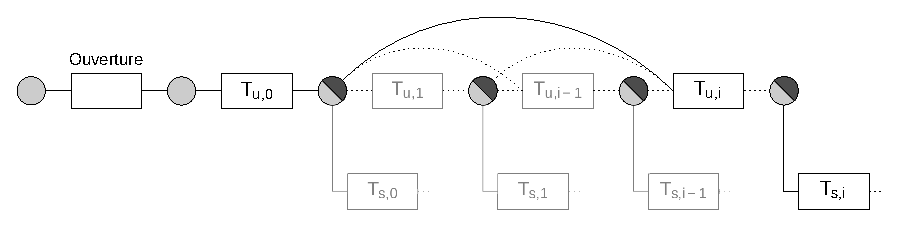
\includegraphics[scale=0.7]{img/eltoo-offchain-protocol.eps}
  \caption{Aperçu du protocole Eltoo.}
\end{figure}

Une transaction supplémentaire est ajoutée à la chaîne de transactions pour éviter que le délai d'expiration des transactions de règlement $T_{s,i}$ soit atteint et qu'elles soient diffusées sur la chaîne. Cette transaction envoie simplement les fonds vers un compte multisignatures classique, et est signée et diffusée après la signature des premières transactions de mise à jour et de règlement ($T_{u,0}$ et $T_{s,0}$). Le délai d'expiration ne commence que lorsque la transaction $T_{u,0}$ est diffusée.

Ce fonctionnement permet d'obtenir un protocole simple de mise à jour du canal, peu contraignant pour les nœuds, sans mécanisme de punition, et permettant de ne pas à avoir à décider les frais à l'avance. Cette facilité d'implémentation pourrait rendre plus aisée la création de contrats plus complexes sur Lightning, comme les canaux de paiement à 3 participants ou plus. En outre, leur implémentation de doit en aucun remplacer celle des canaux de Poon-Dryja~: les deux modèles peuvent coexister au sein d'un seul et même réseau de canaux de paiement.

Les transactions flottantes sont implémentées à l'aide de \texttt{SIGHASH\_ALL | SIGHASH\_ANYPREVOUT}. \textcolor{darkgray}{La mise en œuvre de Eltoo repose donc sur l'intégration du BIP-118 à Bitcoin.}

\section*{L'inscription de données arbitraires}
\addcontentsline{toc}{section}{L'inscription de données arbitraires}

% Données arbitraire
Bitcoin permet d'inscrire des données non financières sur la chaîne, c'est-à-dire des données qui ne sont pas nécessaires dans le blocage et dans la rédemption des fonds et qui sont interprétées de manière extérieure. Même en imposant toutes les restrictions possibles, on ne pourrait pas empêcher l'inscription de ces données, même si on pourrait la rendre plus coûteuse.

% Laisser sa marque pour la postérité
La chaîne de blocs est largement partagée autour du monde, et sera conservée par l'humanité, au moins comme un reliquat historique, de sorte qu'on peut supposer que ce qui y est stocké sera conservé très longtemps. Cette caractéristique pousse les gens à chercher à y inclure des choses qui leur tiennent à cœur. Il est dans la nature de l'homme de chercher à laisser des traces de son passage sur Terre et écrire sur la chaîne principale de Bitcoin est une manière de le faire.

% Méthodes d'inscription
Il existe diverses méthodes d'inscription, qui ont chacune leurs qualités et leurs défauts. Celles-ci ont évolué au fur et à mesure des années, alors que cette utilisation se libéralisait\sendnote{Andrew Sward, Ivy Vecna, Forrest Stonedahl, \eng{Data Insertion in Bitcoin's Blockchain}, 3 avril 2018~: \url{https://doi.org/10.5195/ledger.2018.101}.}.

% Inscription dans la base de pièce par les mineurs
D'une part, l'écriture de données arbitraires peut être réalisée par les mineurs au sein de la base de pièce, l'entrée de transaction de récompense. C'est cette méthode dont Satoshi Nakamoto a fait usage pour inscrire le désormais célèbre titre de une du Times du 3 janvier 2009 dans le bloc de genèse~:

\begin{Verbatim}[fontsize=\footnotesize]
The Times 03/Jan/2009 Chancellor on brink of second bailout for banks
\end{Verbatim}

% Inscriptions par les mineurs
D'autres blocs contiennent des messages emblématiques. Le bloc d'exode de BCH contenait un message de bienvenue pour Shuya Yang, la fille du PDG de la coopérative ViaBTC\sendnote{Bitcoin Cash, bloc 478~559~: «~\eng{Welcome to the world, Shuya Yang!}~».}. Le bloc 629~999, le bloc précédant le troisième halving sur BTC en 2020, contenait le titre d'un article du New York Times du 9 avril annonçant l'injection de liquidité record de la Réserve Fédérale (2~300 milliars de dollars) en réaction à la crise du Covid-19\sendnote{Bitcoin-BTC, bloc 629~999~: «~\eng{NYTimes 09/Apr/2020 With \$2.3T Injection, Fed's Plan Far Exceeds 2008 Rescue}~»}.

Le champ de la base de pièce peut être utilisé pour écrire d'autres données. C'est le cas du nonce supplémentaire (le critère qui a permis d'identifier les bitcoins de Satoshi\sendnote{Sergio Lerner, \eng{The Well Deserved Fortune of Satoshi Nakamoto, Bitcoin creator, Visionary and Genius}, 17 avril 2013~: \url{https://bitslog.com/2013/04/17/the-well-deserved-fortune-of-satoshi-nakamoto/}.}). C'est aussi le cas du signalement des coopératives minières qui est réalisé dans ce champ~: par exemple, la base de pièce du bloc 751~005 contient la chaîne de caractères \texttt{poolin.com}, ce qui indique que sa validation a probablement été réalisée par la coopérative chinoise Poolin.

% Inscription par les utilisateurs
D'autre part, le privilège d'écrire des données arbitraires sur la chaîne n'est pas réservé aux mineurs. Les simples utilisateurs peuvent aussi le faire à condition de payer les frais correspondants.

% Stockage dans les sorties transactionnelles (P2PKH, P2MS et P2SH)
Avant 2014, on procédait la plupart du temps à ces inscriptions en stockant les données dans les scripts de verrouillage, par exemple par l'utilisation de l'instruction de dépilement \texttt{OP\_DROP}\sendnote{La transaction \longstring{c0b2cf75b47d1e7f48cdb4287109ff1dd5bcf146d5f77a9e8784c0c9c0ef02ad}, confirmée le 13 décembre 2012, contient par exemple la chaîne de caractères \texttt{TheCakeIsALie\textbackslash{}n} en référence au jeu vidéo Portal.}. Une autre pratique courante était d'inscrire les données dans les sorties de type P2PKH qui étaient rendues indépensables au passage. Cette méthode était extrêmement coûteuse en raison de la forme de la transaction (imposant l'inscription dans les sorties transactionnelles) et le fait de devoir envoyer des montants non nuls en sortie. Elle était également dommageable pour le système dans son ensemble, car elle encombrait l'ensemble des UTXO.

% Instruction OP_RETURN (première utilisation en mars 2013 : 1a2e22a717d626fc5db363582007c46924ae6b28319f07cb1b907776bd8293fc)
En mars 2014, l'arrivée de la version 0.9.0 de Bitcoin Core a rendu standarde l'instruction \texttt{OP\_RETURN}, dont l'effet est de mettre fin à l'exécution du script\sendnote{L'instruction \texttt{OP\_RETURN} servait initialement à retourner la valeur au sommet de la pile, d'où son nom. Cependant, en juillet 2010, la découverte du «~\eng{1 RETURN bug}~», qui permettait de dépenser toute sortie transactionnelle via le script de déverrouillage \texttt{TRUE RETURN}, a poussé Satoshi Nakamoto à désactiver cette fonctionnalité en lui faisant renvoyer \texttt{FALSE} systématiquement (\url{https://github.com/bitcoin/bitcoin/commit/a75560d828464c3f1138f52cf247e956fc8f937d}).}. Ce changement permettait de créer «~une sortie assurément élagable, pour éviter les schémas de stockage de données [...] qui stockaient des données arbitraires telles que des images en tant que sorties transactionnelles éternellement indépensables, gonflant ainsi la base de données des UTXO de bitcoin\sendnote{\eng{Bitcoin Core version 0.9.0 released}, 19 mars 2014~: \url{https://bitcoin.org/en/release/v0.9.0\#opreturn-and-data-in-the-block-chain}.}~». % "The OP_RETURN change creates a provably-prunable output, to avoid data storage schemes – some of which were already deployed – that were storing arbitrary data such as images as forever-unspendable TX outputs, bloating bitcoin's UTXO database."

\textbf{NULLDATA} Le schéma résultant, appelé NULLDATA (signifiant littéralement «~données insignifiantes~»), est désormais un moyen standard d'inscrire des informations sur la chaîne dans une limite de 80~octets par transaction\sendnote{Dans BTC, la taille des données suivant \texttt{OP\_RETURN} est de \textcolor{darkgray}{83 octets} (règle de mempool), donnant la possibilité d'inscription de 80 octets de données arbitraires.}. Il est identifié par la présence de l'opérateur \texttt{OP\_RETURN} suivi de données empilées~:

\begin{Verbatim}[fontsize=\small]
RETURN [données arbitraires]
\end{Verbatim}

Ce type de sortie est exempt de la limite standarde de poussière, qui est \textcolor{darkgray}{actuellement de 546 satoshis pour les sorties P2PKH}, de façon à pouvoir créer une sortie de 0 satoshis et ne pas gaspiller des fonds inutilement.

% Stockage dans les entrées transactionnelles : P2SH, P2WPKH, P2WSH, P2TR
En outre, il est aussi possible de stocker des données au sein des entrées transactionnelles ou des les témoins liés, lors de la dépense de sorties P2SH, P2WSH ou P2TR. Cette écriture peut se faire dans les scripts de récupération ou bien dans les éléments de déverrouillage. Cette méthode a l'avantage de ne pas surcharger l'ensemble des UTXO. Côté utilisateur, dans où SegWit s'applique, elle a pour bénéfice de diviser le coût des données arbitraires inscrites dans la transactions par quatre.

% --- Inscriptions ---

Ces différentes méthodes ont été utilisées pour inscrire toutes sortes de choses sur la chaîne, dont notamment des empreintes cryptographiques, du texte et des images\sendnote{Ken Shirriff, \eng{Hidden surprises in the Bitcoin blockchain and how they are stored: Nelson Mandela, Wikileaks, photos, and Python software}, 16 février 2014~: \url{https://www.righto.com/2014/02/ascii-bernanke-wikileaks-photographs.html}.}.

% Horodatage par inscription d'empreintes
D'abord, on peut inscrire une empreinte, l'inscription servant alors à l'horodatage. Il s'agit d'inscrire l'empreinte d'un fichier sur la chaîne en tant que preuve d'existence. Cette idée a été mise en avant en février 2009 par Hal Finney dans un de ses courriels adressés à la liste de diffusion dédiée à Bitcoin. Il suggérait alors que «~la pile de blocs de bitcoin serait parfaite~» pour «~prouver qu'un certain document a existé à un certain moment dans le passé\sendnote{Hal Finney, \eng{Re: [bitcoin-list] Bitcoin v0.1.5 released}, \wtime{27/02/2009 20:00:12 UTC}, archive~: \url{https://web.archive.org/web/20131016004925/http://sourceforge.net/p/bitcoin/mailman/bitcoin-list/?viewmonth=200902}.}~», un point de vue approuvé par Satoshi\sendnote{«~En effet, Bitcoin est un serveur d'horodatage sécurisé et distribué pour les transactions. Quelques lignes de code pourraient créer une transaction avec une empreinte supplémentaire de tout ce qui doit être horodaté. Je devrais ajouter une commande pour horodater un fichier de cette façon.~» -- Satoshi Nakamoto, \eng{Re: [bitcoin-list] Bitcoin v0.1.5 released}, \wtime{04/03/2009 16:59:12 UTC}, archive~: \url{https://web.archive.org/web/20131016004648/http://sourceforge.net/p/bitcoin/mailman/bitcoin-list/?viewmonth=200903}.}. % "BTW I don't remember if we talked about this, but the other day some people were mentioning secure timestamping. You want to be able to prove that a certain document existed at a certain time in the past. Seems to me that bitcoin's stack of blocks would be perfect for this." -- "Indeed, Bitcoin is a distributed secure timestamp server for transactions.  A few lines of code could create a transaction with an extra hash in it of anything that needs to be timestamped. I should add a command to timestamp a file that way."

En somme, cette pratique permet de démontrer la connaissance d'une information avant sa publication, et donc indirectement qu'on en est l'auteur probable. Ce type d'usage est notamment mis en œuvre par l'entreprise française Woleet.

% Empreintes pour IPFS
Cet usage peut aussi être exploité par les systèmes décentralisés d'hébergement de fichiers, comme le système IPFS (InterPlanetary File System) qui utiliser les empreintes des fichiers pour les identifier et permettre leur stockage par un réseau pair-à-pair d'utilisateurs. Il est donc possible d'associer le texte écrit sur la chaîne de blocs et des images ou des vidéos, hébergées de manière décentralisée.

% Texte
Ensuite, on peut inscrire un texte, qui est généralement encodé en ASCII~/~UTF-8. Par exemple, la phrase «~Il est possible d'écrire des données arbitraires sur toutes les chaînes.~» a été inscrite sur la chaîne de BTC le 3 décembre 2019\sendnote{Transaction d'identifiant \longstring{9f4482bf9a8ac9233eef676e7746787cc420620f855f97643ea812a53ca561a3}.}. L'inscription de textes permet aussi de dessiner des images en art ASCII. C'est le cas de l'hommage à Len Sassaman, décédé en juillet 2011, qui a été inscrit sur la chaîne par les développeurs Dan Kaminsky et Travis Goodspeed par le biais de sorties P2PKH\sendnote{Cet hommage peut être retrouvé dans la transaction d'identifiant \longstring{930a2114cdaa86e1fac46d15c74e81c09eee1d4150ff9d48e76cb0697d8e1d72} confirmée le 30 juillet 2011.}, et qui contient notamment une représentation du président de la Fed d'alors, Ben Bernanke~:

\begin{Verbatim}[fontsize=\small]
---BEGIN TRIBUTE---  =-=-=-=-=-=-=-=-=-=     ASCII BERNANKE
#./BitLen            LEN "rabbi" SASSAMA  :'::.:::::.:::.::.:
:::::::::::::::::::       1980-2011       : :.: ' ' ' ' : :':
:::::::.::.::.:.:::  Len was our friend.  :.:     _.__    '.:
:.: :.' ' ' ' ' : :  A brilliant mind,    :   _,^"   "^x,   :
:.:'' ,,xiW,"4x, ''  a kind soul, and     '  x7'        `4,
:  ,dWWWXXXXi,4WX,   a devious schemer;    XX7            4XX
' dWWWXXX7"     `X,  husband to Meredith   XX              XX
 lWWWXX7   __   _ X  brother to Calvin,    Xl ,xxx,   ,xxx,XX
:WWWXX7 ,xXX7' "^^X  son to Jim and       ( ' _,+o, | ,o+,"
lWWWX7, _.+,, _.+.,  Dana Hartshorn,       4   "-^' X "^-'" 7
:WWW7,. `^"-" ,^-'   coauthor and          l,     ( ))     ,X
 WW",X:        X,    cofounder and         :Xx,_ ,xXXXxx,_,XX
 "7^^Xl.    _(_x7'   Shmoo and so much      4XXiX'-___-`XXXX'
 l ( :X:       __ _  more.  We dedicate      4XXi,_   _iXX7'
 `. " XX  ,xxWWWWX7  this silly hack to     , `4XXXXXXXXX^ _,
  )X- "" 4X" .___.   Len, who would have    Xx,  ""^^^XX7,xX
,W X     :Xi  _,,_   found it absolutely  W,"4WWx,_ _,XxWWX7'
WW X      4XiyXWWXd  hilarious.           Xwi, "4WW7""4WW7',W
"" ,,      4XWWWWXX  --Dan Kaminsky,      TXXWw, ^7 Xk 47 ,WH
, R7X,       "^447^  Travis Goodspeed     :TXXXWw,_ "), ,wWT:
R, "4RXk,      _, ,  P.S.  My apologies,  ::TTXXWWW lXl WWT:
TWk  "4RXXi,   X',x  BitCoin people.  He  ----END TRIBUTE----
lTWk,  "4RRR7' 4 XH  also would have
:lWWWk,  ^"     `4   LOL'd at BitCoin's
::TTXWWi,_  Xll :..  new dependency upon
\end{Verbatim}

% Images
Enfin, on peut inscrire une image, qui peut être encodée dans de multiples formats, dont notamment en JPEG ou en PNG. Un logo Bitcoin datant du 13 mai 2011 peut être retrouvé\sendnote{Transactions \longstring{ceb1a7fb57ef8b75ac59b56dd859d5cb3ab5c31168aa55eb3819cd5ddbd3d806} et \longstring{9173744691ac25f3cd94f35d4fc0e0a2b9d1ab17b4fe562acc07660552f95518}}. Un hommage à Nelson Mandela accompagné d'une photo a été publié le 7 décembre 2013, quelques jours après sa mort\sendnote{Transactions \longstring{8881a937a437ff6ce83be3a89d77ea88ee12315f37f7ef0dd3742c30eef92dba}.}. En 2022, l'absence de restriction standarde sur la taille des scripts de Taproot a permis de réaliser des inscriptions volumineuses d'une manière bien plus transparente et directe. C'est ce qui a notamment permis d'inscrire l'image des Taproot Wizards qui pesait quasiment 4~Mo (voir figure~\ref{fig:taproot-wizards}).

\begin{figure}[h]
  \centering
  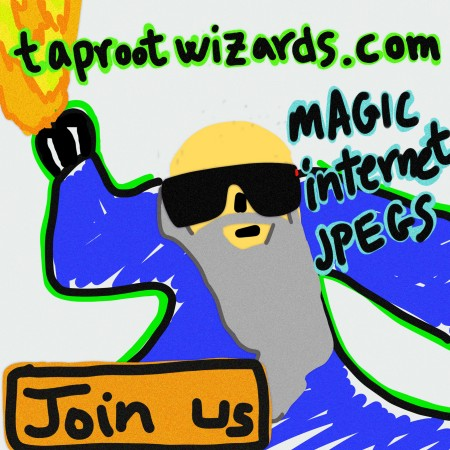
\includegraphics[scale=0.6]{img/taproot-wizards-small-0301e0480b374b32851a9462db29dc19fe830a7f7d7a88b81612b9d42099c0aei0.jpg}
  \caption{Image (réduite) des Taproot Wizards.}
  \label{fig:taproot-wizards}
\end{figure}

% Autres fichiers
De manière générale, tout format de fichier peut être stocké sur la chaîne au travers de transactions multiples~: un document\sendnote{Le PDF du livre blanc de Bitcoin a été inscrit sous forme de sorties P2MS au sein de la transaction \longstring{54e48e5f5c656b26c3bca14a8c95aa583d07ebe84dde3b7dd4a78f4e4186e713}, le 6 avril 2013.}, un livre, une vidéo, un jeu\sendnote{Nicholas Carlini, \eng{Yet Another Doom Clone}, 1\ier{} février 2023~: \url{https://ordinals.com/inscription/521f8eccffa4c41a3a7728dd012ea5a4a02feed81f41159231251ecf1e5c79dai0}, \url{https://nicholas.carlini.com/writing/2019/javascript-doom-clone-game.html}.}, etc.

% Pertinence de cet usage
Cependant, cet usage n'est pas forcément toujours pertinent. L'inscription demande le paiement de frais, parfois élevés, et n'est pas franchement fait pour conserver des données volumineuses. La publication sur IPFS et sur serveur local est généralement bien plus opportune.

% Bitcoin SV
La communauté de Bitcoin SV s'est spécialisée dans cette utilisation, considérant que son registre était une «~source universelle de vérité\sendnote{CoinGeek, \eng{Jerry Chan: Bitcoin’s value is as a universal source of truth}, 17 juillet 2019~: \url{https://coingeek.com/jerry-chan-bitcoins-value-is-as-a-universal-source-of-truth-video/}.}~». Ainsi, on peut retrouver un volume assez importants de données météorologiques sur sa chaîne, qui y sont inscrites depuis 2019\sendnote{Helen Partz, \eng{98\% of BSV Transactions Used for Writing Weather Data on Blockchain: Report}, 24 juin 2019~: \url{https://cointelegraph.com/news/98-of-bsv-transactions-used-for-writing-weather-data-on-blockchain-report}.}.

\section*{Les métaprotocoles}
\addcontentsline{toc}{section}{Les métaprotocoles}

% Définition
Les métaprotocoles sont des protocoles qui se servent du protocole de base pour fonctionner. Ils font usage de l'inscription de données arbitraires sur la chaîne pour inclure des instructions qui sont interprétées par des implémentations logicielles spécifiques\sendnote{C'est en ce sens que les métaprotocoles peuvent être appelés des surcouches, même si on préfère généralement utiliser ce terme pour parler des systèmes comme Lightning par exemple.}. Ils ont pour particularité d'être nécessairement plus extensifs que le protocole de base.

% Bitcoin 2.0
Ce n'est pas une idée nouvelle. Dès les premières années d'existence de Bitcoin, certaines personnes ont été désireuses de l'exploiter plus en profondeur, de se servir de lui d'une autre manière que comme un instrument de transfert de valeur. Ce mouvement initial était appelé «~Bitcoin 2.0~» par certains, et il a par la suite mené à l'élaboration d'Ethereum à partir de 2013.

% Colored Coins
Le premier type de métaprotocole qui a été élaboré est le procédé des \eng{colored coins}, ou pièces colorées en français, qui consiste à marquer des pièces (UTXO) par des données inscrites. Chaque type de jeton créé est liée à un identifiant, que l'on peut assimiler à une couleur, d'où le nom de ce procédé. L'idée est apparue en 2012\sendnote{Yoni Assia, \eng{bitcoin 2.X (aka Colored Bitcoin) – initial specs}, 27 mars 2012~: \url{https://yoniassia.com/coloredbitcoin/}~; Meni Rosenfeld, \eng{Overview of Colored Coins}, 4 décembre 2012~: \url{https://bitcoil.co.il/BitcoinX.pdf}.}. % inscrites notamment par l'utilisation de l'opérateur \texttt{OP\_RETURN}

\textcolor{brown}{schéma colored coin}

% Implémentation des colored coins
L'implémentation de cette idée a été réalisée dès la fin de l'année 2012 par l'intermédiaire du ChromaWallet\sendnote{Alex Mizrahi, \eng{ChromaWallet (colored coins): issue and trade private currencies/stocks/bonds/..}, \wtime{07/09/2012 12:46:12 UTC}~: \url{https://bitcointalk.org/index.php?topic=106373.msg1167516\#msg1167516}.}. Mais elle n'a vraiment pris de l'ampleur qu'à partir de 2014, avec l'apparition des Open Assets de Coinprism, des \eng{CoinSpark assets} de Coin Sciences, et des Colored Coins de Colu. Ces usages sont depuis tombés en désuétude, même si le procédé a pu servir de manière sporadique au fil des années, comme dans le cas du jeton BSQ de Bisq créé en 2018 comme base de sa DAO. Une tentative de restauration a également été faite sur Bitcoin Cash avec les jetons SLP, sans grand succès. % Open Assets (\texttt{OA}), Colored Coins (\texttt{CC}), CoinSpark assets (\texttt{SPK})

% Mastercoin et Counterparty
Au-delà des pièces colorées, il existait également des protocoles plus évolués qui avaient la particularité de gérer une unité de compte propre. Il s'agissait essentiellement de Mastercoin, qui a été renommé en Omni en mars 2015, et de Counterparty.

% Mastercoin, 2013
Le premier métaprotocole de ce type a été Mastercoin\sendnote{Le mot «~master~» dans le nom de Mastercoin est l'acronyme de «~\eng{Metadata Archival by Standard Transaction Embedding Records}~», d'après les spécifications techniques~: \url{https://github.com/OmniLayer/spec/blob/master/OmniSpecification-v0.6.adoc}.}, dont le livre blanc, intitulé «~\eng{The Second Bitcoin Whitepaper}~», a été publié le 6 janvier 2012 par J.R. Willett\sendnote{J.R. Willett, \eng{[It's here] The Second Bitcoin Whitepaper}, \wtime{06/01/2012 22:42:24 UTC}~: \url{https://bitcointalk.org/index.php?topic=56901.msg678427\#msg678427}~; J.R. Willett, \eng{The Second Bitcoin Whitepaper}, 6 janvier 2012~: \url{https://cryptochainuni.com/wp-content/uploads/Mastercoin-2nd-Bitcoin-Whitepaper.pdf}.}. Il s'agissait d'un protocole permettant à ses utilisateurs de créer leurs propres devises, appelées «~\eng{user currencies}~».

% MSC et ICO
Mastercoin reposait sur une unité de compte notée le MSC, qui a fait l'objet d'une prévente d'un mois en juillet-août 2013\sendnote{Tous les bitcoins envoyés à l'adresse \longstring{1EXoDusjGwvnjZUyKkxZ4UHEf77z6A5S4P} étaient transformés en MSC à raison de 100~MSC au début, taux dégressif au fil des semaines. }. C'était la première \eng{Initial Coin Offering} de l'histoire, et elle a recueilli 5120~BTC, soit plus de 500~000~\$ à ce moment-là.

% USDT
Le plus grand succès de ce protocole a probablement été la création du premier stablecoin, le Tether USD, qui a été émis sous le nom de Realcoin en octobre 2014. Mastercoin~/~Omni a longtemps été l'unique manière de posséder et de transférer de l'USDT avant que le jeton ne soit émis massivement sur d'autres chaînes comme Ethereum et Tron.

% Counterparty, 2014
Le second métaprotocole avancé a été Counterparty, lancé en janvier 2014. Cette plateforme reposait également sur un jeton natif, le XCP, qui lui servait de carburant, et qui a été créé par brûlage de bitcoins durant son premier mois d'existence\sendnote{Tous les bitcoins envoyés à l'adresse \longstring{1CounterpartyXXXXXXXXXXXXXXXUWLpVr} entre le 2 janvier et le 3 février 2014 étaient convertis en XCP à un taux qui variait entre 1000 et 1500~XCP par BTC}. Ce sont 2140~bitcoins qui ont ainsi été rendus inutilisables pour donner vie à plus de 2,6~millions de XCP, encore en circulation aujourd'hui. Counterparty se voulait plus flexible que Mastercoin en rendant possible l'implémentation de contrats autonomes, notamment dans le but de créer des jetons et d'héberger des plateformes d'échange décentralisées, appelées des «~distributeurs~».

% Jetons non fongibles (NFT)
En particulier, Counterparty a été la première plateforme à proposer la gestion de jetons non fongibles (NFT). Il s'agissait là de mettre en œuvre une vieille idée, qui avait notamment été mise en valeur par Hal Finney en 1993 sur la liste de diffusion cypherpunk sous la forme de «~cartes à collectionner cryptographiques\sendnote{Hal Finney, \eng{Crypto trading cards.}, \wtime{17/01/1993 18:48:02 UTC}~: \url{https://cypherpunks.venona.com/date/1993/01/msg00152.html}.}~». Counterparty a ainsi hébergé une multitude de collections de tels objets, comme les cartes à jouer de \eng{Spells of Genesis} et de SaruTobi créées en 2015, ou les Rare Papes émis entre 2016 et 2018\sendnote{Vlad Costea, \eng{Bitcoin NFTs On Counterparty (And How To Get Or Create Your First One)}, 29 décembre 2021~: \url{https://bitcoin-takeover.com/bitcoin-nfts-on-counterparty-and-how-to-get-or-create-your-first-one/}.}.

% Memo, 2018
En 2018, l'apparition de Bitcoin Cash a motivé la création d'un média social dont les données seraient entièrement stockées sur la chaîne, les développeurs de BCH étant plus libéraux à ce sujet. Le protocole s'appelait Memo et consistait à publier de courts messages visibles publiquement sous un profil défini et à pouvoir suivre les autres utilisateurs, à aimer et répondre à leurs messages. L'idée était d'obtenir une sorte de réseau social résistant à la censure, mais souffrait néanmoins de la nécessité de payer des frais. \sendnote{Le protocole Memo est disponible à l'adresse~: \url{https://memo.cash/protocol}.}

% Ordinals, 2023
Tous ces protocoles ont perdu de leur jusqu'à l'apparition du protocole Ordinals, lancé en janvier 2023. Ce métaprotocole permettait de créer et de gérer des «~artefacts numériques~», c'est-à-dire de NFT dont l'intégralité des données est stockée de manière immuable sur une chaîne résistante à la censure. Le protocole Ordinals reposait sur une «~théorie des ordinaux~» permettant de suivre et de transférer des satoshis liés à une inscription, comme un texte, un image ou autre chose\sendnote{\url{https://docs.ordinals.com/}}. En particulier, Ordinals a été utilisé pour émuler la propriété et le transfert de jetons fongibles, baptisés «~BRC-20~», dont le succès spéculatif a provoqué une congestion du réseau menant à une hausse des frais de transaction record.

% STAMPS, 2023
Le succès d'Ordinals a également inspiré la création du protocole STAMPS, qui se basait sur Counterparty pour le suivi des artefacts et stockait leurs données dans des sorties P2MS\sendnote{STAMP est l'acronyme de \eng{Secure, Tradeable Art Maintained Permanently}. -- Mike In Space, \eng{STAMPS: A Protocol for Storing Images On-Chain in Transaction Outputs Immutably on Bitcoin}, 6 avril 2023~: \url{https://github.com/mikeinspace/stamps/tree/main}.}.

% Opposition
Toutes ces pratiques ont créé des débats. En effet, Bitcoin était présenté comme un modèle de monnaie numérique et il semblait contreproductif d'en faire un protocole de conservation de données qui ne seraient pas relatives au transfert de bitcoins. Ainsi, dès décembre 2010, Jeff Garzik s'opposait au fait d'utiliser la chaîne pour le stockage généralisé\sendnote{Jeff Garzik, \eng{Resist the urge to use block chain for generalized storage}, \wtime{07/12/2010 22:04:54 UTC}~: \url{https://bitcointalk.org/index.php?topic=2129.msg27884\#msg27884}.}. Plus tard, en 2014, des disputes similaires ont éclaté au sujet de Counterparty\sendnote{BitMEX Research, \eng{The OP\_Return Wars of 2014 – Dapps Vs Bitcoin Transactions}, 12 juillet 2022~: \url{https://blog.bitmex.com/dapps-or-only-bitcoin-transactions-the-2014-debate/}.}. En 2023, c'est également la même discorde qui a eu lieu à la suite du succès d'Ordinals\sendnote{pourteaux, \eng{Illegitimate bitcoin transactions}, 25 janvier 2023~: \url{https://read.pourteaux.xyz/p/illegitimate-bitcoin-transactions}.}.

% Premier défaut : manque de vérification
Ces métaprotocoles ont deux défauts majeurs. Le premier est que la vérification de leurs règles dépend d'un petit sous-ensemble de nœuds du réseau. En effet, la gestion d'un tel protocole construit en surcouche demande des ressources supplémentaires, notamment en ce qui concerne l'indexation pour les pièces colorées. De ce fait, peu de personnes déploient une implémentation complète, ce qui centralise considérablement le protocole et le rendent sensible à la modification par un adversaire, notamment pour y inclure de la censure.

% Second défaut : frais
Le second défaut est leurs frais d'utilisation parfois très élevés, surtout si la limite de capacité transactionnelle du réseau est atteinte. Les transactions mettant en place ces solutions sont nécessairement plus volumineuses que les transactions normales et entraînent par conséquent des frais plus élevés. Elles sont donc plus facilement exclues par l'augmentation des frais issue de la congestion du réseau.

% Conséquences de ces défauts
C'est pour ces raisons que les personnes qui ont travaillé sur ces solution s'en sont vite détournées, préférant se réfugier vers des plateformes alternatives comme NXT et surtout Ethereum. Vitalik Buterin lui-même s'intéressait aux pièces colorées et à Mastercoin en 2013 avant de commencer à bâtir ce qui allait devenir Ethereum\sendnote{Yoni Assia, Vitalik Buterin, Meni Rosenfeld, Rotem Lev, \eng{Colored Coins whitepaper}, 2013~: \url{http://www.ma.senac.br/wp-content/uploads/2018/05/ColoredCoinswhitepaper-DigitalAssets.pdf}~; Vitalik Buterin, \eng{A Prehistory of the Ethereum Protocol}, 14 septembre 2017~: \url{https://vitalik.ca/general/2017/09/14/prehistory.html}.}. C'est aussi pour ces raisons que des solutions moins coûteuses (des surcouches utilisant la chaîne comme un procédé de règlement et non pas comme un lieu où inscrire toutes les opérations) sont aujourd'hui privilégiées pour faire ce genre de choses comme RGB ou Taro.

\section*{Les contrats hors chaîne} % Scriptless Scripts, Taproot et RGB
\addcontentsline{toc}{section}{Les contrats hors chaîne}

% Mise à niveau Schnorr-Taproot
La cryptographie permet de déployer des contrats sans que ceux-ci ne doivent être inscrits sur la chaîne. Cette particularité a été facilitée grâce à la mise à niveau Schnorr-Taproot, souvent appelée simplement Taproot, qui est survenue sur BTC le 14 novembre 2021 et qui incluait deux éléments majeurs~: le schéma de signature de Schnorr et le procédé de programmation de contrats Taproot. Ces fonctionnalités ont été intégrées sous forme d'un soft fork au sein du schéma standard P2TR correspondant à la version 1 de SegWit.

% Schéma de signature de Schnorr
Le schéma de Schnorr implémenté est une dérivation du protocole d'authentification du même nom décrit en 1989 par Claus-Peter Schnorr. Il s'agit d'une alternative à ECDSA qui se base sur la même courbe elliptique (\texttt{secp256k1}) et qui permet de signer des transactions grâce aux mêmes paires de clés.

% Avantages des signatures de Schnorr
Comparé à ECDSA, le schéma de signature de Schnorr possède quelques avantages. Premièrement, il produit des signatures moins grandes. Deuxièmement, les signatures produites sont non-malléables, le procédé ne faisant pas intervenir de nombre aléatoire. Troisièmement, et c'est le plus important, il présente une propriété de linéarité, ce qui permet notamment de faire des choses comme la vérification par lots et l'agrégation des clés. \sendnote{Pieter Wuille, Jonas Nick, Tim Ruffing, \eng{Schnorr Signatures for secp256k1}, 19 janvier 2020~: \url{https://github.com/bitcoin/bips/blob/master/bip-0340.mediawiki}.}

% Pourquoi Schnorr n'a pas été intégré dans Bitcoin
Le schéma de Schnorr est supérieur à ECDSA et existait en 2008, mais Satoshi Nakamoto n'a pas daigné s'en servir. Ce choix s'explique par le fait que l'algorithme était breveté aux États-Unis jusqu'en février 2008 et que par conséquent il n'existait pas d'implémentation standardisée. Le logiciel de Bitcoin utilisait en effet OpenSSL, qui n'intégrait pas ce type d'algorithme.

% Scriptless Scripts
Le schéma de Schnorr autorise le déploiement de \eng{Scriptless Scripts}, de contrats «~sans script~» qui sont exécutés en dehors de la chaîne et appliqués au sein des signatures. Le concept a été théorisé en 2017 par Andrew Poelstra\sendnote{Andrew Poelstra, \eng{Using the Chain for what Chains are Good For}, Scaling Bitcoin IV, 5 novembre 2017~: \url{https://www.youtube.com/watch?v=3pd6xHjLbhs\&t=5755s}~; Aaron van Wirdum, \eng{Scriptless Scripts: How Bitcoin Can Support Smart Contracts Without Smart Contracts}, 27 novembre 2017~: \url{https://bitcoinmagazine.com/technical/scriptless-scripts-how-bitcoin-can-support-smart-contracts-without-smart-contracts}.}. Il se retrouve dans des exemples comme le schéma de multisignature MuSig2\sendnote{Jonas Nick, Tim Ruffing, Yannick Seurin, \eng{MuSig2: Simple Two-Round Schnorr Multi-Signatures}, 14 octobre 2020~: \url{https://eprint.iacr.org/2020/1261.pdf}.}, les \eng{adaptor signatures} ou encore les \eng{Discreet Log Contracts}\sendnote{Thaddeus Dryja, \eng{Discreet Log Contracts}, 2017~: \url{https://adiabat.github.io/dlc.pdf}.}.

% Taproot
Outre cela, le schéma de Schnorr facilite grandement l'implémentation de Taproot, qui a été intégré au protocole au même moment. Taproot (dont le nom signifie littéralement «~racine pivot~» en français) est un système d'arbres syntaxiques abstraits merkélisés permettant d'ancrer les clauses d'un contrat au sein d'un arbre de Merkle et de cacher cet arbre sous une clé publique agrégée appartenant à ses participants. Il permet ainsi de ne publier le contrat qu'en cas de litige, et même dans ce cas, de ne publier que les conditions exécutées\sendnote{Pieter Wuille, Jonas Nick, Anthony Towns, \eng{Taproot: SegWit version 1 spending rules}, 19 janvier 2020~: \url{https://github.com/bitcoin/bips/blob/master/bip-0341.mediawiki}.}. Les scripts utilisés dans Taproot utilisent un langage de programmation nommé Tapscript, basé sur le langage de script classique de Bitcoin\sendnote{Pieter Wuille, Jonas Nick, Anthony Towns, \eng{Validation of Taproot Scripts}, 19 janvier 2020~: \url{https://github.com/bitcoin/bips/blob/master/bip-0342.mediawiki}.}.

% MAST
Un arbre syntaxique abstrait merkélisé (aussi appelés MAST pour \eng{Merklized Abstract Syntax Tree}) est un arbre de hachage (voir chapitre~\ref{ch:confirmation}) qui contient les empreintes des clauses (conditions de dépense). Lors de l'exécution du MAST, l'utilisateur a seulement besoin de révéler la clause appliquée, ce qui lui permet de dépenser les fonds, et de fournir les empreintes liées aux autres conditions sans les dévoiler.

\textcolor{brown}{schéma MAST : 5 clauses, fermeture coopérative multisig 5-parmi-5 (bonne pratique) et autres conditions}

% Historique
L'implémentation des MAST au sein de Bitcoin avait déjà été proposée par le passé, que ce soit sous la forme d'une nouvelle version de SegWit (BIP-114), ou bien d'un nouvel code opération \texttt{OP\_MERKLEBRANCHVERIFY} (BIP-116, BIP-117). Mais Taproot a constitué une proposition supérieure en permettant de ne pas révéler l'existence du MAST lui-même.

% Racine pivot
Taproot autorise la dépense coopérative par la modification légère (\eng{tweaking}) de la clé publique agrégée interne à l'aide de la racine du MAST. La clé obtenue est celle inscrite dans le script de verrouillage de la pièce, de sorte qu'elle est indiscernable des autres sorties P2TR. De même, la signature agrégée est indiscernable d'une signature classique. Taproot constitue ainsi une façon de régler les contrats en dehors de la chaîne, tant qu'il n'y a pas de litige.

% RGB
Au-delà de Taproot, une alternative est RGB, qui est un système de contrats autonomes hors chaîne, construit à la fois en surcouche de Bitcoin et de Lightning. Le nom est issu du standard RGB (\eng{Red Green Blue}) qui permet de définir une couleur et constitue par conséquent une référence directe aux \eng{colored coins}, RGB ayant été originellement conçu comme «~une meilleure version des pièces colorées\sendnote{RGB FAQ, \eng{What does 'RGB' stand for?}, 14 décembre 2020~: \url{https://www.rgbfaq.com/faq/what-does-rgb-stand-for}.}~». Cependant, même si RBG permet effectivement d'émettre et de gérer des jetons, cette fonctionnalité est loin d'être la seule.

RGB se base sur deux primitives techniques conceptualisées en 2016 par le développeur Peter Todd\sendnote{\url{https://petertodd.org/2016/state-machine-consensus-building-blocks#uniqueness-and-single-use-seals}~; \url{https://petertodd.org/2016/closed-seal-sets-and-truth-lists-for-privacy}.}~: la validation côté client (\eng{client-side validation}) et les scellés à usage unique (\eng{single-use seals}). Cela permet la gestion d'un état indépendant, pour lequel la double dépense est empêchée par ces scellés. Après fait l'objet de recherches par Giacomo Zucco et le BHB Network, RGB est actuellement développé par la LNP/BP Standards Association.

% Avantages généraux
L'implémentation de contrats en dehors de la chaîne est donc possible sur Bitcoin. Et ils apportent deux choses. D'une part, ils réduisent le paiement de frais en ayant une empreinte minimale sur la chaîne. D'autre part, ils améliorent la confidentialité de leurs participants. C'est pourquoi ils pourraient jouer un grand rôle à l'avenir.

\section*{Une monnaie programmable}
\addcontentsline{toc}{section}{Une monnaie programmable}

L'aspect programmable de Bitcoin est souvent négligé. Il n'est en effet pas directement présenté dans le livre blanc, bien que Satoshi Nakamoto l'avait déjà élaboré. Toutefois, il est capital et constitue l'une des facettes de Bitcoin.

La programmabilité de la monnaie peut servir à contrôler, comme c'est le cas dans les projets de MNBC qui fleurissent autour du monde. Mais elle peut également rendre un fier service à la liberté individuelle. En effet, cette aspect modulable donne l'occasion à des personnes qui ne se connaissent pas d'échanger de la valeur de la façon la plus sûre possible ou, comme l'exprimait Tim May dans son \emph{Manifeste crypto anarchiste} en 1988, de «~faire des affaires et négocier des contrats électroniques sans jamais connaître le Vrai Nom, ou l'identité légale, de l'autre\sendnote{Timothy C. May, \eng{The Crypto Anarchist Manifesto}, \wtime{22/11/1992 20:11:24 UTC}~: \url{https://cypherpunks.venona.com/date/1992/11/msg00204.html}.}~».

Les contrats autonomes forment donc la pierre angulaire des relations financières dans le cyberespace. Même la communauté de Monero, qui avait particulièrement restreint cet aspect à des fins de confidentialité, est revenu sur ses pas en intégrant au protocole la possibilité pour la multisignature, notamment dans le but de permettre les échanges atomiques.

\printendnotes